% ============================================================
% CI-0131 Diseño de Experimentos – Laboratorio 2
% ============================================================
\documentclass[11pt,a4paper]{article}

% --- Encoding & language ---
\usepackage[utf8]{inputenc}
\usepackage[T1]{fontenc}
\usepackage[spanish]{babel}

% --- Font: Times New Roman ---
\usepackage{mathptmx}

% --- Geometry ---
\usepackage[top=2.5cm, bottom=2.5cm, left=3cm, right=3cm]{geometry}

% --- Graphics ---
\usepackage{graphicx}
\usepackage{float}

% --- Tables ---
\usepackage{booktabs}
\usepackage{array}
\usepackage{longtable}

% --- Code listings ---
\usepackage{listings}
\usepackage{xcolor}

\definecolor{codebg}{rgb}{0.95,0.95,0.95}
\definecolor{codeframe}{rgb}{0.7,0.7,0.7}
\definecolor{codecomment}{rgb}{0.3,0.6,0.3}
\definecolor{codestring}{rgb}{0.7,0.1,0.1}
\definecolor{codekeyword}{rgb}{0.1,0.1,0.7}

\lstdefinestyle{Rstyle}{
  language=R,
  backgroundcolor=\color{codebg},
  frame=single,
  rulecolor=\color{codeframe},
  basicstyle=\ttfamily\small,
  keywordstyle=\color{codekeyword}\bfseries,
  stringstyle=\color{codestring},
  commentstyle=\color{codecomment}\itshape,
  breaklines=true,
  breakatwhitespace=true,
  showstringspaces=false,
  tabsize=2,
  numbers=none,
  captionpos=b,
}

\lstdefinestyle{Routput}{
  backgroundcolor=\color{white},
  frame=single,
  rulecolor=\color{codeframe},
  basicstyle=\ttfamily\footnotesize,
  breaklines=true,
  breakatwhitespace=true,
  showstringspaces=false,
  numbers=none,
  captionpos=b,
}

% --- Misc ---
\usepackage{parskip}
\usepackage{hyperref}
\hypersetup{colorlinks=true, linkcolor=blue, urlcolor=blue}
\usepackage{enumitem}
\usepackage{tcolorbox}

% Question box
\tcbuselibrary{skins}
\newtcolorbox{pregunta}{
  colback=yellow!10!white,
  colframe=orange!80!black,
  fonttitle=\bfseries,
  title={Pregunta y Respuesta},
  left=6pt, right=6pt, top=4pt, bottom=4pt
}

% ============================================================
\begin{document}

% ============================================================
% PORTADA
% ============================================================
\begin{titlepage}
  \centering
  \vspace*{2cm}
  {\Large \textbf{Universidad de Costa Rica} \par}
  \vspace{0.5cm}
  {\large Escuela de Ciencias de la Computación e Informática \par}
  \vspace{1.5cm}
  \rule{\linewidth}{0.5pt}\\[0.4cm]
  {\LARGE \textbf{CI-0131 --- Diseño de Experimentos} \par}
  \vspace{0.3cm}
  {\Large Ciclo I -- 2026 \par}
  \rule{\linewidth}{0.5pt}\\[1cm]
  {\Huge \textbf{Laboratorio \#2} \par}
  \vspace{0.5cm}
  {\Large \textit{Análisis Exploratorio de Datos y Gráficos Depurados} \par}
  \vspace{2cm}
  {\large \textbf{Profesor:} Ignacio Díaz Oreiro \par}
  \vspace{2cm}
  {\large \textbf{Estudiante(s):} \par}
  \vspace{0.4cm}
  {\large Christopher Zuniga \hspace{1cm} (czuniga28) \par}
  \vfill
  {\large \today \par}
\end{titlepage}

% ============================================================
\tableofcontents
\newpage

% ============================================================
\section{Introducción}
% ============================================================

El análisis exploratorio de datos (EDA, por sus siglas en inglés) es un proceso que permite la identificación
de las tendencias dentro de los conjuntos de los datos. Durante el desarrollo de un experimento es importante
que se logre identificar la presencia de algunas de estas tendencias o medidas como la existencia de valores
faltantes, valores extremos, medidas de valores centrales o de dispersión. Esta información valiosa nos da
acceso a relevante conocimiento acerca de nuestro conjunto de datos.

La presencia de valores faltantes puede indicar que durante la recolección de datos algo no fue tan riguroso
como se planteó, o bien que exista algún sesgo en el conjunto de datos, lo que potencialmente puede
evidenciarse mediante un análisis visual. La presencia de valores extremos podría ser un indicador de posibles
errores de muestreo o de la consecución de datos.

En este laboratorio se trabaja con el conjunto de datos de Pokémon disponible en Kaggle
(\url{https://www.kaggle.com/datasets/rounakbanik/pokemon}), que contiene 801 Pokémon con 40 variables
que describen sus características estadísticas, tipo, generación y estado de legendario. El objetivo es
aplicar técnicas de EDA para identificar patrones, valores faltantes y distribuciones en las variables más
relevantes.

El laboratorio se divide en dos partes: la primera realiza un EDA con gráficos y tablas básicas utilizando
las funcionalidades nativas de R y la biblioteca \texttt{ggplot2}; la segunda parte genera visualizaciones
más depuradas utilizando librerías adicionales como \texttt{dplyr}, \texttt{gridExtra}, \texttt{reshape2}
y \texttt{RColorBrewer}.

% ============================================================
\section{Parte A: Análisis Exploratorio de Datos}
% ============================================================

\subsection{A.1 Información General}

Para comenzar el análisis se carga el conjunto de datos \texttt{pokemon.csv} utilizando la función
\texttt{read.csv()}, indicando que el archivo contiene encabezados (\texttt{header = TRUE}) y
especificando la codificación UTF-8 para garantizar el manejo correcto de caracteres especiales.
Posteriormente se utiliza \texttt{attach(df)} para poder referenciar las columnas directamente por su nombre.

\begin{lstlisting}[style=Rstyle, caption={Carga del conjunto de datos}]
df <- read.csv("pokemon.csv", header = TRUE, encoding = "UTF-8")
attach(df)
\end{lstlisting}

El dataset contiene \textbf{801 filas} (Pokémon) y \textbf{40 columnas} (variables).

\subsubsection{Estadísticas descriptivas con summary()}

La función \texttt{summary()} proporciona las medidas de tendencia central y dispersión de cada variable
numérica: mínimo, primer cuartil, mediana, media, tercer cuartil y máximo. También indica la cantidad
de valores faltantes (\texttt{NA's}) cuando los hay.

\textbf{Variable: attack}

Se presentan a continuación las estadísticas descriptivas de la variable \texttt{attack}, que representa
el poder de ataque físico de cada Pokémon.

\begin{lstlisting}[style=Rstyle]
summary(df$attack)
\end{lstlisting}

\begin{lstlisting}[style=Routput]
   Min. 1st Qu.  Median    Mean 3rd Qu.    Max.
   5.00   55.00   75.00   77.86  100.00  185.00
\end{lstlisting}

\textbf{Variable: defense}

La variable \texttt{defense} representa la resistencia al daño físico de cada Pokémon.

\begin{lstlisting}[style=Rstyle]
summary(df$defense)
\end{lstlisting}

\begin{lstlisting}[style=Routput]
   Min. 1st Qu.  Median    Mean 3rd Qu.    Max.
   5.00   50.00   70.00   73.01   90.00  230.00
\end{lstlisting}

\textbf{Variable: hp}

La variable \texttt{hp} (hit points) representa los puntos de vida de cada Pokémon.

\begin{lstlisting}[style=Rstyle]
summary(df$hp)
\end{lstlisting}

\begin{lstlisting}[style=Routput]
   Min. 1st Qu.  Median    Mean 3rd Qu.    Max.
   1.00   50.00   65.00   68.96   80.00  255.00
\end{lstlisting}

\textbf{Variable: weight\_kg}

La variable \texttt{weight\_kg} indica el peso en kilogramos de cada Pokémon.

\begin{lstlisting}[style=Rstyle]
summary(df$weight_kg)
\end{lstlisting}

\begin{lstlisting}[style=Routput]
   Min. 1st Qu.  Median    Mean 3rd Qu.    Max.    NA's
   0.10    9.00   27.30   61.38   64.80  999.90      20
\end{lstlisting}

\textbf{Variable: height\_m}

La variable \texttt{height\_m} indica la altura en metros de cada Pokémon.

\begin{lstlisting}[style=Rstyle]
summary(df$height_m)
\end{lstlisting}

\begin{lstlisting}[style=Routput]
   Min. 1st Qu.  Median    Mean 3rd Qu.    Max.    NA's
  0.100   0.600   1.000   1.164   1.500  14.500      20
\end{lstlisting}

\begin{pregunta}
\textbf{¿Encontró algunos valores faltantes? ¿En qué variables?}\\[4pt]
Sí. Se encontraron \textbf{20 valores faltantes (NA)} en las variables \texttt{weight\_kg} y
\texttt{height\_m}. Las variables \texttt{attack}, \texttt{defense} y \texttt{hp} no presentan
valores faltantes. Esto puede indicar que para algunos Pokémon no se registró o no se pudo determinar
con certeza su peso o altura en el momento de la recolección de datos, o bien que se trató de un
error de transcripción en el dataset.
\end{pregunta}

\subsubsection{Tablas de contingencia para variables categóricas}

Las tablas de contingencia (usando \texttt{table()}) permiten conocer la distribución de
frecuencias de variables categóricas.

\textbf{Tabla de contingencia: type1}

Se muestra la cantidad de Pokémon por tipo primario.

\begin{lstlisting}[style=Rstyle]
table(df$type1)
\end{lstlisting}

\begin{lstlisting}[style=Routput]
     bug   dark dragon electric  fairy fighting  fire flying
      72     29     27       39     18       28    52      3
   ghost  grass ground    ice normal  poison psychic   rock
      27     78     32     23    105      32      53     45
   steel  water
      24    114
\end{lstlisting}

\textbf{Tabla de contingencia: type2}

Se muestra la cantidad de Pokémon por tipo secundario. La primera categoría (384) corresponde a
Pokémon que no tienen tipo secundario.

\begin{lstlisting}[style=Rstyle]
table(df$type2)
\end{lstlisting}

\begin{lstlisting}[style=Routput]
              bug   dark dragon electric  fairy fighting   fire
     384        5     21     17        9      29       25     13
  flying  ghost  grass ground    ice normal  poison psychic
      95     14     20     34     15      4      34      29
    rock  steel  water
      14     22     17
\end{lstlisting}

\textbf{Tabla de contingencia: is\_legendary}

\begin{lstlisting}[style=Rstyle]
table(df$is_legendary)
\end{lstlisting}

\begin{lstlisting}[style=Routput]
  0   1
731  70
\end{lstlisting}

\textbf{Tabla de contingencia: generation}

\begin{lstlisting}[style=Rstyle]
table(df$generation)
\end{lstlisting}

\begin{lstlisting}[style=Routput]
  1   2   3   4   5   6   7
151 100 135 107 156  72  80
\end{lstlisting}

\subsubsection{Conversión a factor y uso de summary()}

R permite tratar variables categóricas como factores con la función \texttt{as.factor()}, lo cual
le indica al intérprete que la variable es cualitativa. Esto modifica los valores en el data frame y
permite usar \texttt{summary()} para obtener tablas de frecuencias equivalentes a las de contingencia.

\begin{lstlisting}[style=Rstyle]
# Para type1 (ejemplo provisto en el enunciado)
df$type1 <- as.factor(df$type1)
summary(df$type1)
\end{lstlisting}

\begin{lstlisting}[style=Routput]
     bug   dark dragon electric  fairy fighting   fire flying
      72     29     27       39     18       28     52      3
   ghost  grass ground    ice normal  poison psychic   rock
      27     78     32     23    105      32      53     45
   steel  water
      24    114
\end{lstlisting}

Se construye de manera equivalente para las demás variables categóricas:

\begin{lstlisting}[style=Rstyle]
df$type2       <- as.factor(df$type2)
df$generation  <- as.factor(df$generation)
df$is_legendary <- as.factor(df$is_legendary)

summary(df$type2)
\end{lstlisting}

\begin{lstlisting}[style=Routput]
              bug   dark dragon electric  fairy fighting   fire
     384        5     21     17        9      29       25     13
  flying  ghost  grass ground    ice normal  poison psychic
      95     14     20     34     15      4      34      29
    rock  steel  water
      14     22     17
\end{lstlisting}

\begin{lstlisting}[style=Rstyle]
summary(df$generation)
\end{lstlisting}

\begin{lstlisting}[style=Routput]
  1   2   3   4   5   6   7
151 100 135 107 156  72  80
\end{lstlisting}

\begin{lstlisting}[style=Rstyle]
summary(df$is_legendary)
\end{lstlisting}

\begin{lstlisting}[style=Routput]
  0   1
731  70
\end{lstlisting}

\subsubsection{Tablas de contingencia cruzadas}

Las tablas de contingencia también permiten clasificar información para dos variables simultáneamente.
A continuación se muestra la distribución de Pokémon legendarios y no legendarios por generación.

\begin{lstlisting}[style=Rstyle]
table(df$generation, df$is_legendary)
\end{lstlisting}

\begin{lstlisting}[style=Routput]
   is_legendary
      0   1
  1 146   5
  2  94   6
  3 125  10
  4  94  13
  5 143  13
  6  66   6
  7  63  17
\end{lstlisting}

\begin{lstlisting}[style=Rstyle]
table(df$is_legendary, df$generation)
\end{lstlisting}

\begin{lstlisting}[style=Routput]
   generation
      1   2   3   4   5   6   7
  0 146  94 125  94 143  66  63
  1   5   6  10  13  13   6  17
\end{lstlisting}

\begin{pregunta}
\textbf{¿Cuáles son los 3 grupos más numerosos de esa última tabla?}\\[4pt]
Analizando la tabla \texttt{table(is\_legendary, generation)}, los tres grupos más numerosos son:\\
\begin{enumerate}
  \item \textbf{Generación 1, no legendarios:} 146 Pokémon
  \item \textbf{Generación 5, no legendarios:} 143 Pokémon
  \item \textbf{Generación 3, no legendarios:} 125 Pokémon
\end{enumerate}
Esto refleja que las tres generaciones con mayor cantidad de Pokémon introducidos son la 1, 5 y 3 respectivamente,
todas con una alta proporción de Pokémon no legendarios.
\end{pregunta}

A continuación se construyen las cuatro tablas que combinan tipo primario con generación, tipo
secundario con generación, tipo primario con estado legendario, y tipo secundario con estado legendario.

\begin{lstlisting}[style=Rstyle]
# type1 con generation
table(df$type1, df$generation)
\end{lstlisting}

\begin{lstlisting}[style=Routput]
           1  2  3  4  5  6  7
  bug     12 10 12  8 18  3  9
  dark     0  5  4  3 13  3  1
  dragon   3  0  7  3  7  4  3
  electric 9  6  4  7  7  3  3
  fairy    2  5  0  1  0  9  1
  fighting 7  2  4  2  7  3  3
  fire    12  8  6  5  8  8  5
  flying   0  0  0  0  1  2  0
  ghost    3  1  4  6  5  4  4
  grass   12  9 12 13 15  5 12
  ground   8  3  6  4  9  0  2
  ice      2  4  6  3  6  2  0
  normal  22 15 18 17 17  4 12
  poison  14  1  3  6  2  2  4
  psychic  8  7  8  7 14  3  6
  rock     9  4  8  6  6  8  4
  steel    0  2  9  3  4  4  2
  water   28 18 24 13 17  5  9
\end{lstlisting}

\begin{lstlisting}[style=Rstyle]
# type2 con generation
table(df$type2, df$generation)
\end{lstlisting}

\begin{lstlisting}[style=Routput]
           1  2  3  4  5  6  7
          70 51 69 53 81 31 29
  bug      0  0  2  1  0  0  2
  dark     4  1  6  4  3  2  1
  dragon   0  1  2  3  3  5  3
  electric 1  2  0  0  4  0  2
  fairy    3  3  5  1  2  4 11
  fighting 1  1  3  5  8  1  6
  fire     1  2  0  0  8  0  2
  flying  19 19 12 14 17  6  8
  ghost    0  0  2  2  4  4  2
  grass    2  1  5  2  5  4  1
  ground   8  7  7  6  2  2  2
  ice      7  1  0  3  1  2  1
  normal   0  0  0  0  0  4  0
  poison  21  3  2  2  5  0  1
  psychic  6  3 12  2  1  3  2
  rock     2  3  4  1  4  0  0
  steel    2  2  0  7  8  0  3
  water    4  0  4  1  0  4  4
\end{lstlisting}

\begin{lstlisting}[style=Rstyle]
# type1 con is_legendary
table(df$type1, df$is_legendary)
\end{lstlisting}

\begin{lstlisting}[style=Routput]
           is_legendary
              0   1
  bug        69   3
  dark       26   3
  dragon     20   7
  electric   34   5
  fairy      17   1
  fighting   28   0
  fire       47   5
  flying      2   1
  ghost      26   1
  grass      74   4
  ground     30   2
  ice        21   2
  normal    102   3
  poison     32   0
  psychic    36  17
  rock       41   4
  steel      18   6
  water     108   6
\end{lstlisting}

\begin{pregunta}
\textbf{De los Pokémon tipo 1, ¿cuál es el grupo más numeroso de Pokémon legendarios?}\\[4pt]
De acuerdo con la tabla \texttt{table(type1, is\_legendary)}, el grupo más numeroso de Pokémon
legendarios de tipo primario es \textbf{psychic (psíquico)} con \textbf{17 Pokémon legendarios}.
Le siguen dragon con 7, steel y water con 6 cada uno. Esto tiene sentido dado que muchos de los
Pokémon legendarios más icónicos de la serie (como Mewtwo, Lugia, Deoxys) son de tipo psíquico.
\end{pregunta}

\begin{lstlisting}[style=Rstyle]
# type2 con is_legendary
table(df$type2, df$is_legendary)
\end{lstlisting}

\begin{lstlisting}[style=Routput]
           is_legendary
              0   1
             359  25
  bug          5   0
  dark        21   0
  dragon      13   4
  electric     8   1
  fairy       23   6
  fighting    19   6
  fire        11   2
  flying      85  10
  ghost       12   2
  grass       18   2
  ground      33   1
  ice         14   1
  normal       4   0
  poison      33   1
  psychic     25   4
  rock        14   0
  steel       18   4
  water       16   1
\end{lstlisting}

\subsubsection{Tablas con tapply() y dplyr}

La función \texttt{tapply()} permite aplicar una función a subconjuntos de datos agrupados por
una variable categórica. A continuación se calcula la media de HP por generación.

\begin{lstlisting}[style=Rstyle]
tapply(df$hp, df$generation, mean)
\end{lstlisting}

\begin{lstlisting}[style=Routput]
       1        2        3        4        5        6        7
64.34437 70.98000 65.66667 73.10280 70.31410 71.11111 70.57500
\end{lstlisting}

Con la biblioteca \texttt{dplyr} es posible obtener resultados equivalentes presentados como tibbles.
Se construyen dos tablas para la media de \texttt{weight\_kg} por generación: la primera removiendo
los valores faltantes y la segunda sin removerlos.

\begin{lstlisting}[style=Rstyle]
library(dplyr)

# Con na.rm = TRUE (removiendo NAs)
df %>%
  group_by(generation) %>%
  summarise(mean_weight_kg = mean(weight_kg, na.rm = TRUE))
\end{lstlisting}

\begin{lstlisting}[style=Routput]
# A tibble: 7 x 2
  generation mean_weight_kg
  <fct>               <dbl>
1 1                    45.8
2 2                    49.1
3 3                    67.1
4 4                    76.9
5 5                    52.4
6 6                    52.2
7 7                    98.3
\end{lstlisting}

\begin{lstlisting}[style=Rstyle]
# Sin na.rm (sin remover NAs)
df %>%
  group_by(generation) %>%
  summarise(mean_weight_kg = mean(weight_kg))
\end{lstlisting}

\begin{lstlisting}[style=Routput]
# A tibble: 7 x 2
  generation mean_weight_kg
  <fct>               <dbl>
1 1                    NA
2 2                    49.1
3 3                    67.1
4 4                    76.9
5 5                    52.4
6 6                    NA
7 7                    NA
\end{lstlisting}

\begin{pregunta}
\textbf{¿Qué pasa cuando una columna sí tiene NAs y no se remueven al construir la tabla?}\\[4pt]
Cuando la columna contiene valores faltantes (\texttt{NA}) y no se utiliza \texttt{na.rm = TRUE},
R propaga el \texttt{NA} en el cálculo: cualquier operación aritmética que incluya un \texttt{NA}
retorna \texttt{NA}. Esto se puede observar en las generaciones 1, 6 y 7, que presentan Pokémon
sin peso registrado: la media resulta \texttt{NA} en lugar de un número. Por esta razón es
fundamental siempre verificar la presencia de valores faltantes antes de calcular estadísticas.
\end{pregunta}

% ============================================================
\subsection{A.2 Histogramas}

Los histogramas permiten visualizar la distribución de variables continuas. Se generaron histogramas
para las variables \texttt{hp}, \texttt{attack}, \texttt{defense}, \texttt{weight\_kg} y
\texttt{height\_m}.

\textbf{Histograma de HP}

La variable \texttt{hp} presenta una distribución asimétrica hacia la derecha, con la mayoría de
los Pokémon concentrados entre 45 y 90 puntos de vida.

\begin{lstlisting}[style=Rstyle]
hist(df$hp, main = "Distribucion de variable HP",
     xlab = "HP", col = "lightblue", border = "black")
\end{lstlisting}

\begin{figure}[H]
  \centering
  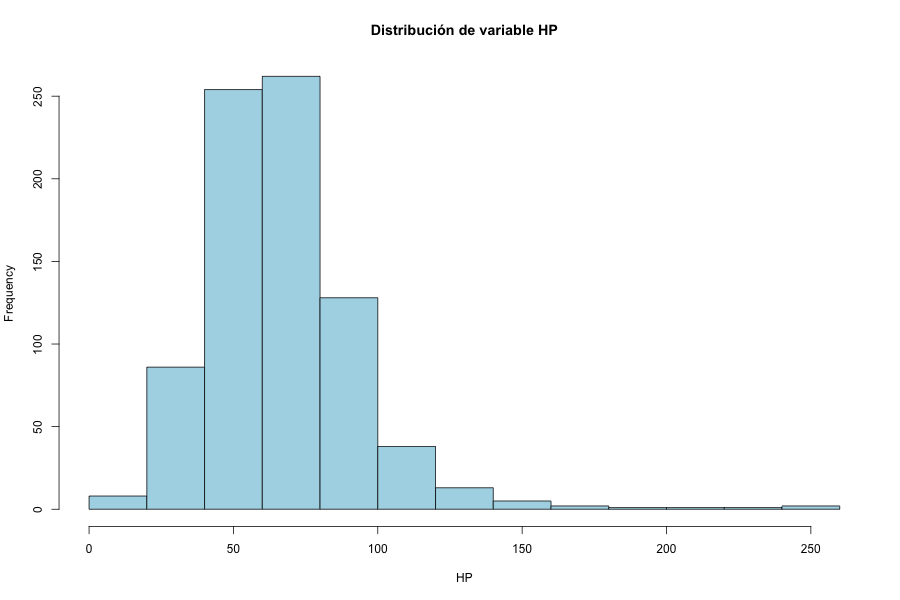
\includegraphics[width=0.85\textwidth]{plots/hist_hp.png}
  \caption{Histograma de la variable HP (puntos de vida) de los Pokémon.}
\end{figure}

\textbf{Histograma de Attack}

La variable \texttt{attack} muestra una distribución aproximadamente simétrica con un ligero sesgo
positivo, centrada alrededor de los 75 puntos de ataque.

\begin{lstlisting}[style=Rstyle]
hist(df$attack, main = "Distribucion de variable Attack",
     xlab = "Attack", col = "lightcoral", border = "black")
\end{lstlisting}

\begin{figure}[H]
  \centering
  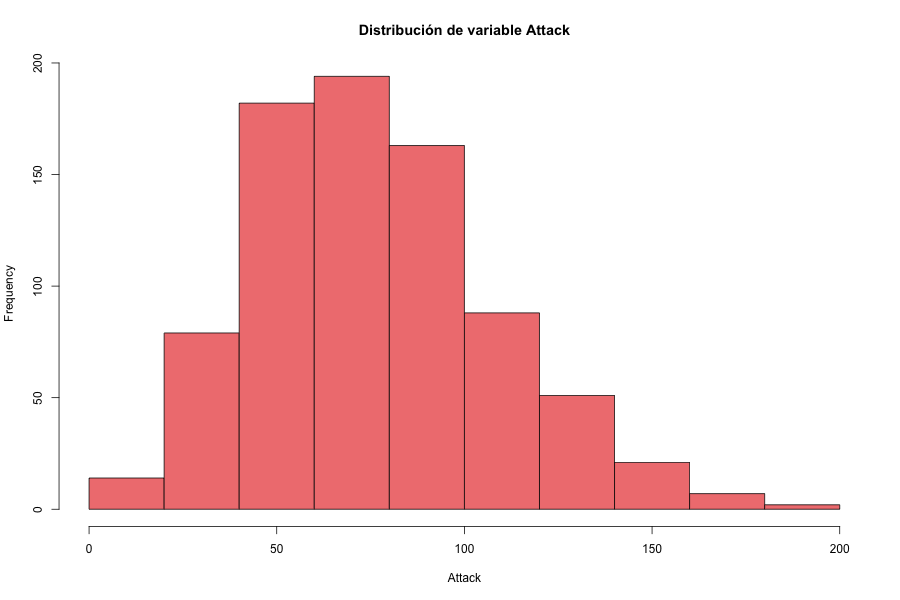
\includegraphics[width=0.85\textwidth]{plots/hist_attack.png}
  \caption{Histograma de la variable Attack (ataque físico) de los Pokémon.}
\end{figure}

\textbf{Histograma de Defense}

La variable \texttt{defense} tiene una distribución asimétrica positiva, con la mayoría de los
valores entre 40 y 100.

\begin{lstlisting}[style=Rstyle]
hist(df$defense, main = "Distribucion de variable Defense",
     xlab = "Defense", col = "lightgreen", border = "black")
\end{lstlisting}

\begin{figure}[H]
  \centering
  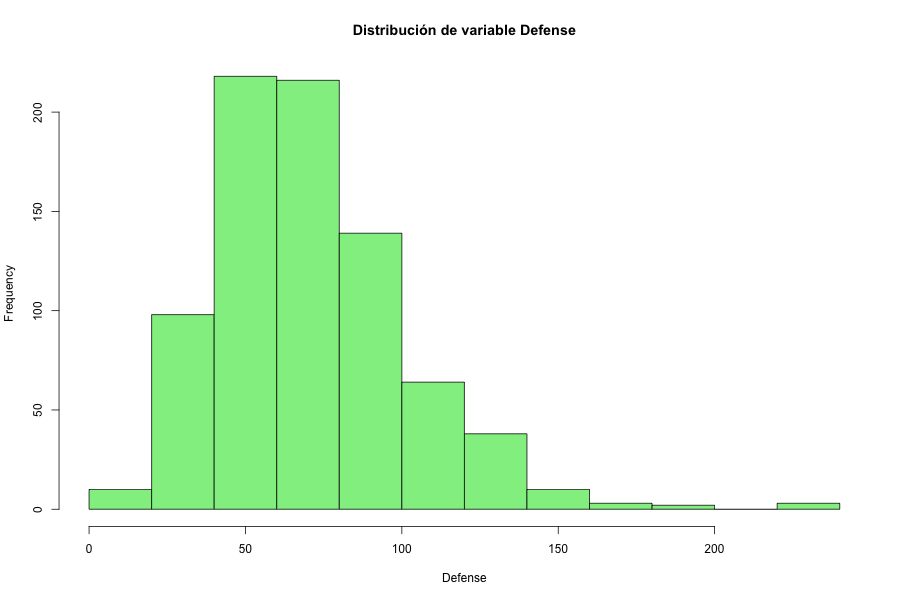
\includegraphics[width=0.85\textwidth]{plots/hist_defense.png}
  \caption{Histograma de la variable Defense (defensa física) de los Pokémon.}
\end{figure}

\textbf{Histograma de Weight (kg)}

La distribución de \texttt{weight\_kg} presenta una marcada asimetría positiva con valores extremos
que superan los 900 kg (como Primal Groudon con 999.9 kg).

\begin{lstlisting}[style=Rstyle]
hist(df$weight_kg, main = "Distribucion de variable Weight (kg)",
     xlab = "Weight (kg)", col = "lightyellow", border = "black")
\end{lstlisting}

\begin{figure}[H]
  \centering
  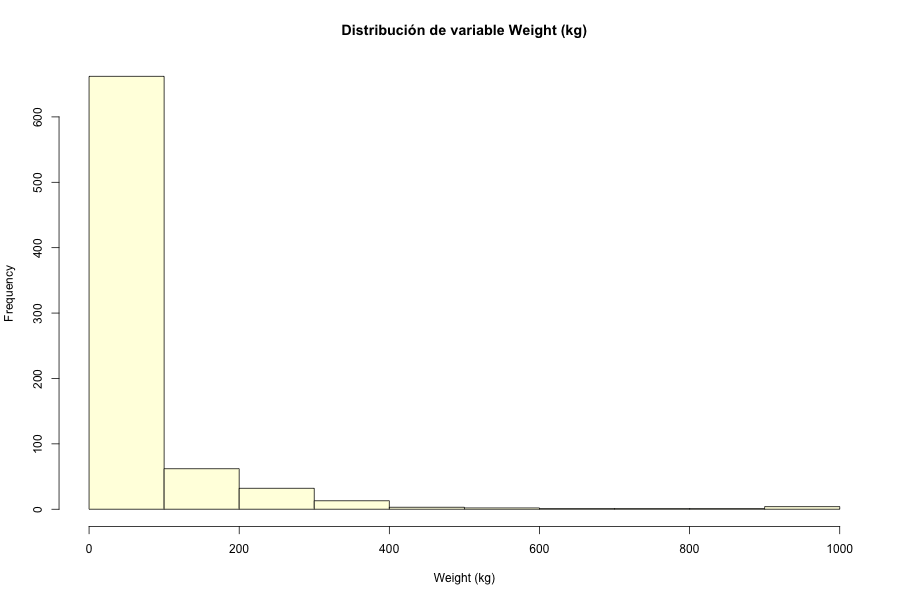
\includegraphics[width=0.85\textwidth]{plots/hist_weight_kg.png}
  \caption{Histograma de la variable Weight\_kg (peso en kilogramos) de los Pokémon.}
\end{figure}

\textbf{Histograma de Height (m)}

La variable \texttt{height\_m} también muestra una distribución muy asimétrica hacia la derecha,
con la gran mayoría de Pokémon midiendo entre 0.5 y 2 metros.

\begin{lstlisting}[style=Rstyle]
hist(df$height_m, main = "Distribucion de variable Height (m)",
     xlab = "Height (m)", col = "plum", border = "black")
\end{lstlisting}

\begin{figure}[H]
  \centering
  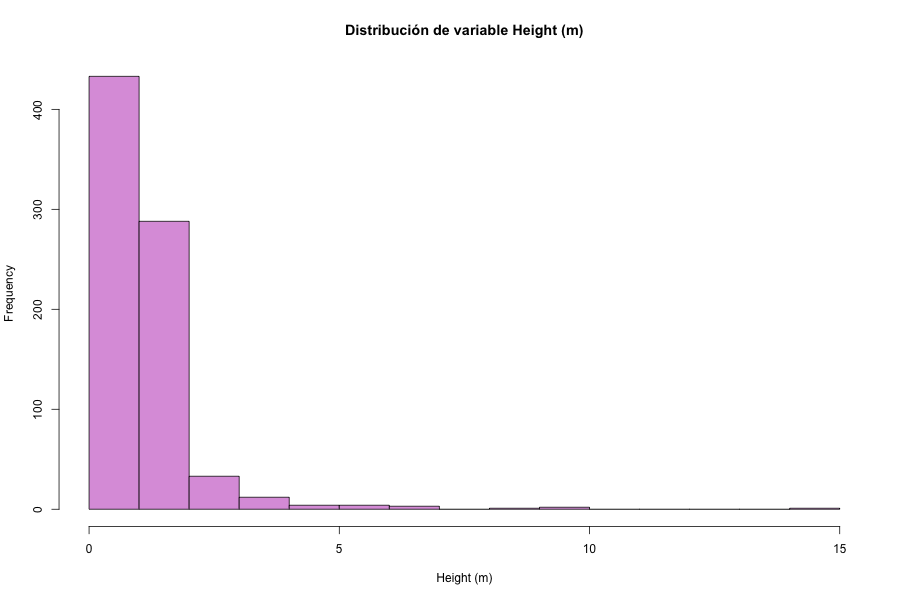
\includegraphics[width=0.85\textwidth]{plots/hist_height_m.png}
  \caption{Histograma de la variable Height\_m (altura en metros) de los Pokémon.}
\end{figure}

% ============================================================
\subsection{A.3 Gráficos de Barras}

Los gráficos de barras permiten visualizar la distribución de variables discretas o categóricas.
Se utilizó \texttt{ggplot2} con la geometría \texttt{geom\_bar()} para todas las variables.

\textbf{Gráfico de barras: type1}

El siguiente gráfico, provisto en el enunciado, muestra la distribución de Pokémon según su
tipo primario. Los tipos más frecuentes son \textbf{water} (114), \textbf{normal} (105) y
\textbf{grass} (78).

\begin{lstlisting}[style=Rstyle]
ggplot(pokemon, aes(x = type1)) +
  geom_bar() +
  theme(axis.text.x = element_text(angle = 45, hjust = 1))
\end{lstlisting}

\begin{figure}[H]
  \centering
  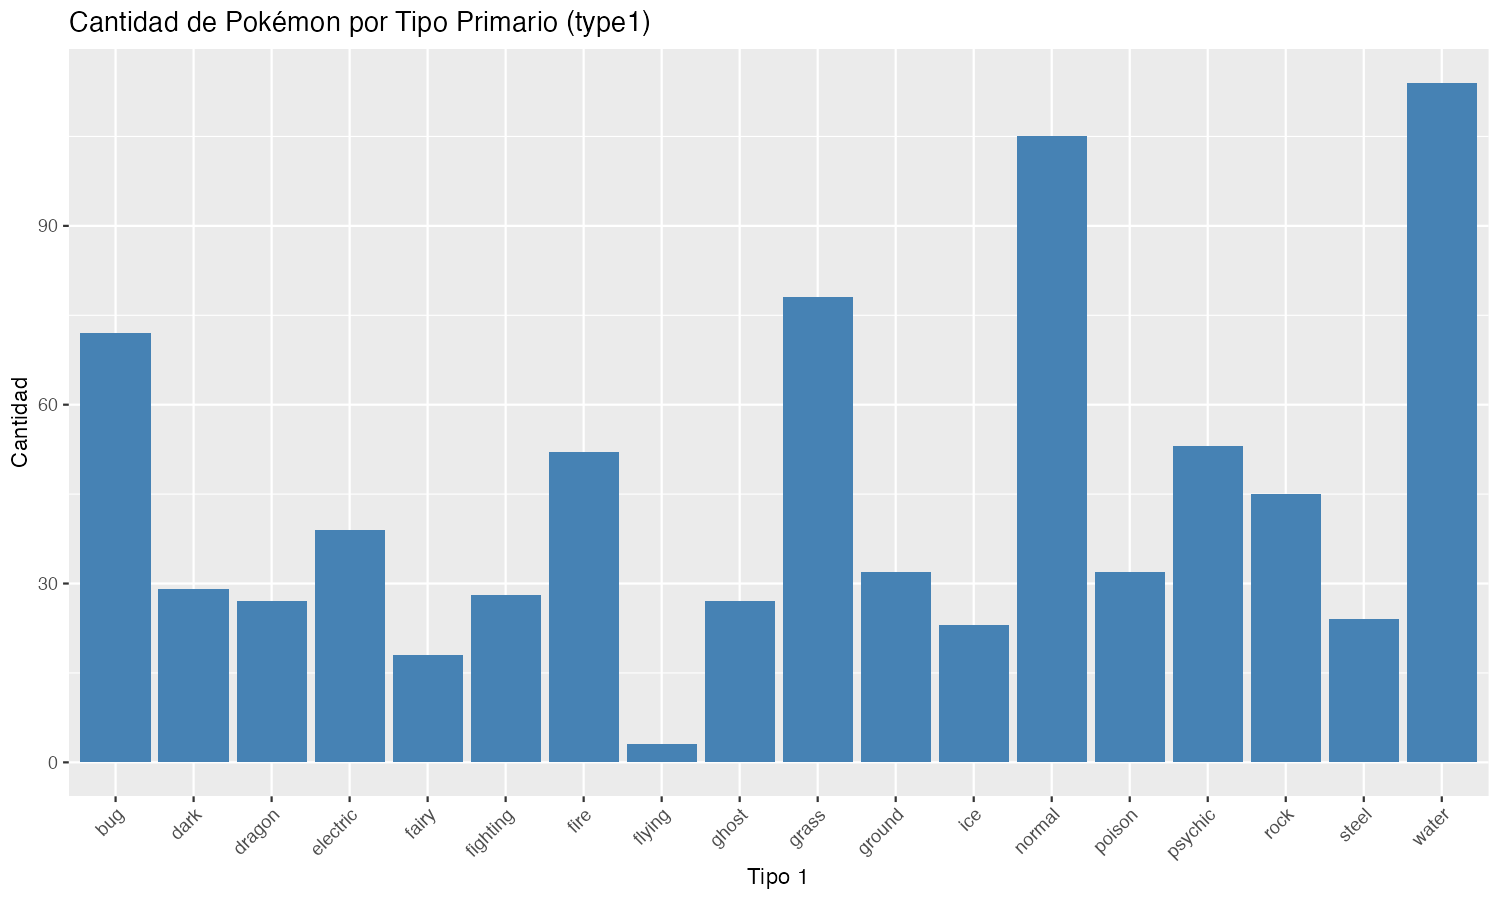
\includegraphics[width=0.95\textwidth]{plots/bar_type1.png}
  \caption{Cantidad de Pokémon por tipo primario (type1).}
\end{figure}

\textbf{Gráfico de barras: type2}

La gran mayoría de Pokémon (384) no posee tipo secundario (barra vacía). Entre los que sí tienen
tipo 2, el más frecuente es \textbf{flying} (95), seguido de \textbf{ground} y \textbf{poison}
(34 cada uno).

\begin{lstlisting}[style=Rstyle]
ggplot(pokemon, aes(x = type2)) +
  geom_bar(fill = "tomato") +
  theme(axis.text.x = element_text(angle = 45, hjust = 1)) +
  labs(title = "Cantidad de Pokemon por Tipo Secundario (type2)",
       x = "Tipo 2", y = "Cantidad")
\end{lstlisting}

\begin{figure}[H]
  \centering
  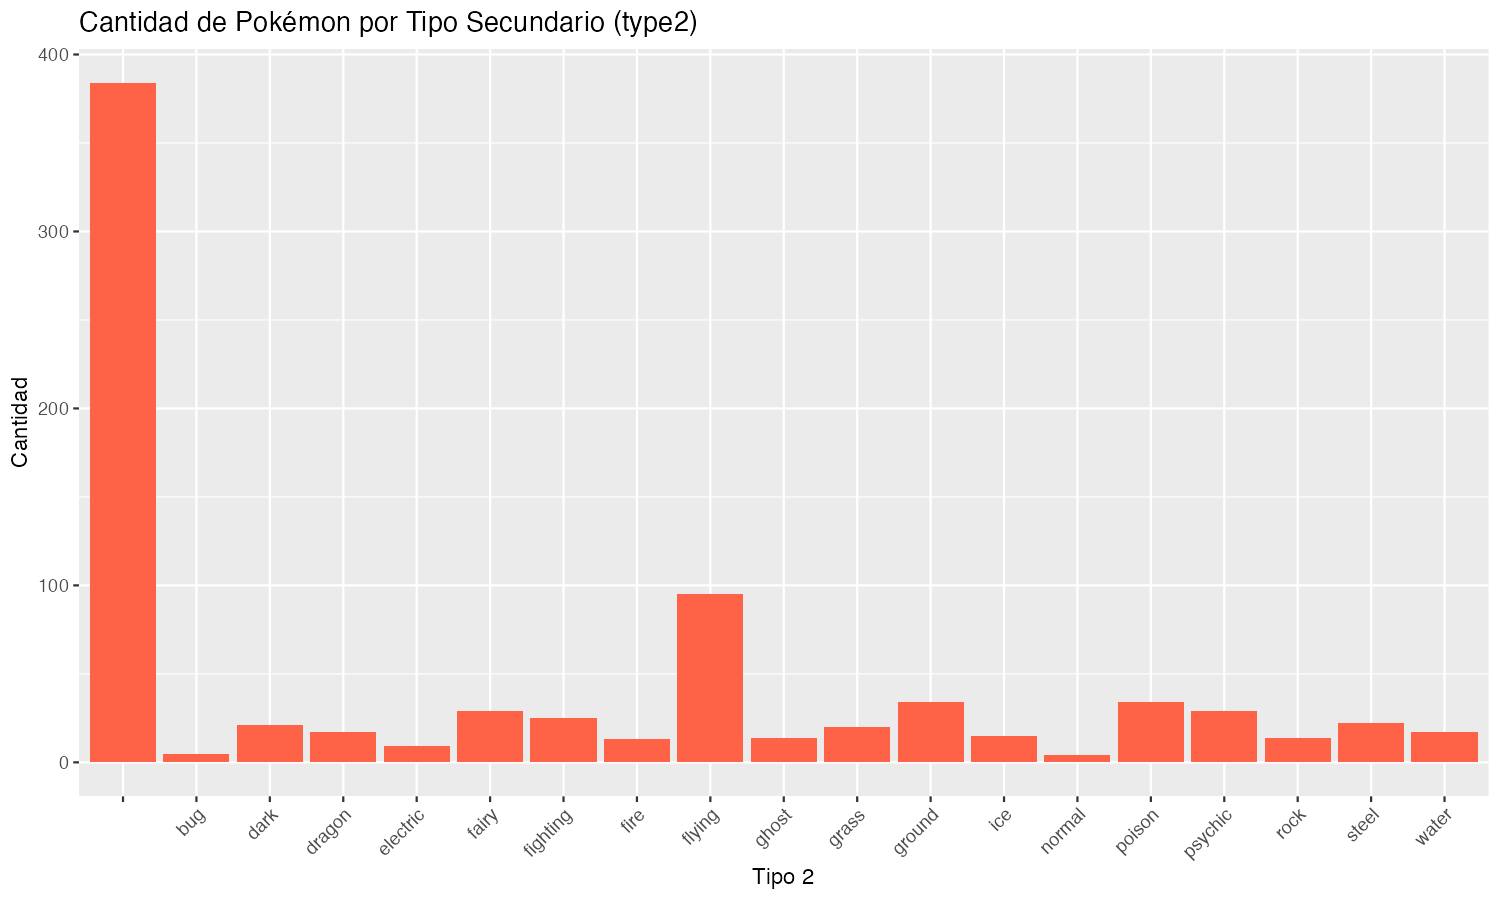
\includegraphics[width=0.95\textwidth]{plots/bar_type2.png}
  \caption{Cantidad de Pokémon por tipo secundario (type2). La barra vacía representa Pokémon sin tipo secundario.}
\end{figure}

\textbf{Gráfico de barras: is\_legendary}

El conjunto de datos está muy desbalanceado: \textbf{731} Pokémon son no legendarios (0) y
\textbf{70} son legendarios (1), lo que representa apenas el 8.7\% del total.

\begin{lstlisting}[style=Rstyle]
ggplot(pokemon, aes(x = is_legendary)) +
  geom_bar(fill = "goldenrod") +
  labs(title = "Cantidad de Pokemon Legendarios vs No Legendarios",
       x = "Es Legendario (0 = No, 1 = Si)", y = "Cantidad")
\end{lstlisting}

\begin{figure}[H]
  \centering
  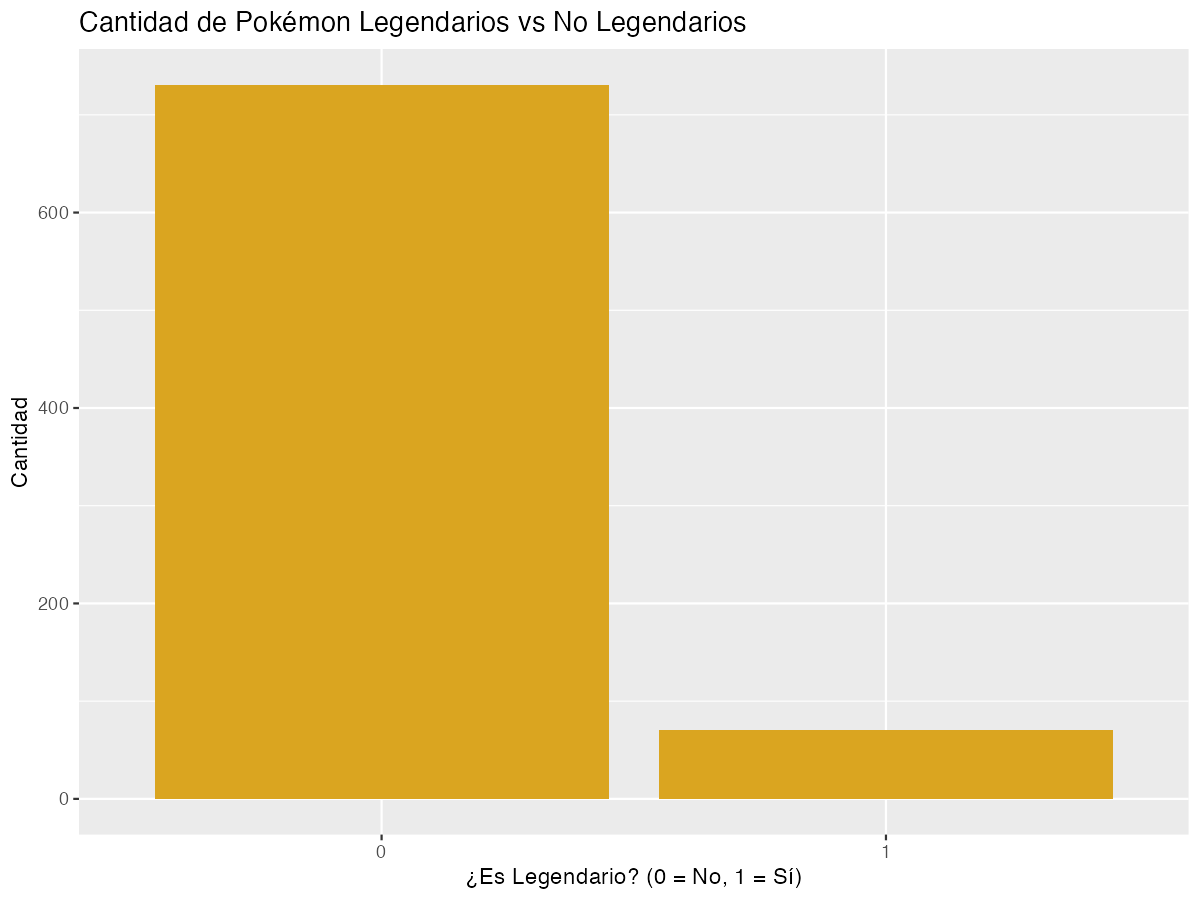
\includegraphics[width=0.75\textwidth]{plots/bar_is_legendary.png}
  \caption{Distribución de Pokémon legendarios (1) vs no legendarios (0).}
\end{figure}

\textbf{Gráfico de barras: generation}

La generación 5 es la que tiene más Pokémon (156), seguida de la generación 1 (151) y la generación
3 (135). La generación 6 es la que menos Pokémon tiene (72).

\begin{lstlisting}[style=Rstyle]
ggplot(pokemon, aes(x = generation)) +
  geom_bar(fill = "mediumseagreen") +
  labs(title = "Cantidad de Pokemon por Generacion",
       x = "Generacion", y = "Cantidad")
\end{lstlisting}

\begin{figure}[H]
  \centering
  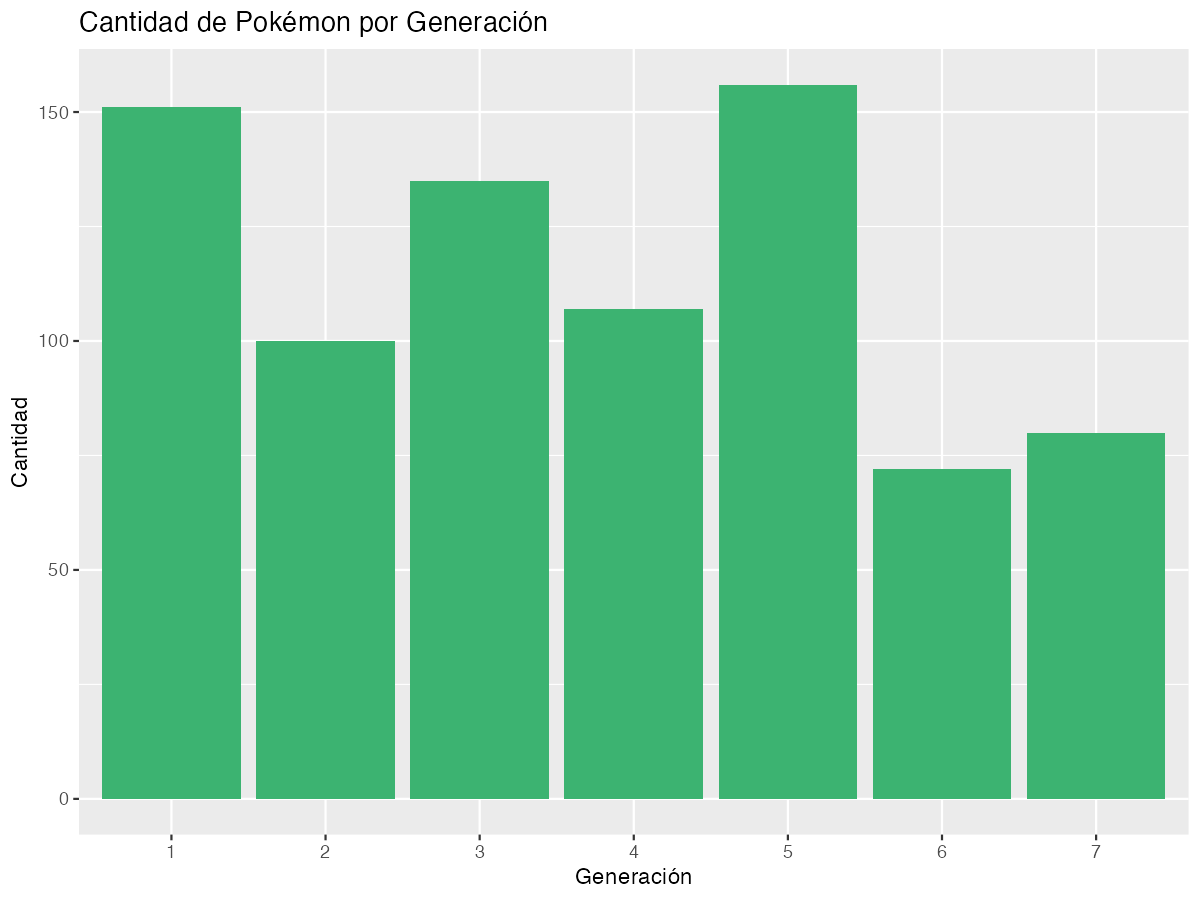
\includegraphics[width=0.75\textwidth]{plots/bar_generation.png}
  \caption{Cantidad de Pokémon por generación.}
\end{figure}

% ============================================================
\subsection{A.4 Boxplots}

Los diagramas de caja (boxplots) permiten comparar la distribución de variables continuas a través
de distintos grupos categóricos, mostrando mediana, cuartiles y valores atípicos.

\textbf{Boxplot: Attack vs Type1}

El siguiente gráfico es el provisto en el enunciado. Permite observar que los tipos \textbf{dragon}
y \textbf{fighting} tienden a tener los valores de ataque más altos, mientras que los tipos
\textbf{fairy} y \textbf{psychic} tienen los más bajos en general.

\begin{lstlisting}[style=Rstyle]
ggplot(pokemon, aes(x = type1, y = attack)) +
  geom_boxplot() +
  theme(axis.text.x = element_text(angle = 45, hjust = 1))
\end{lstlisting}

\begin{figure}[H]
  \centering
  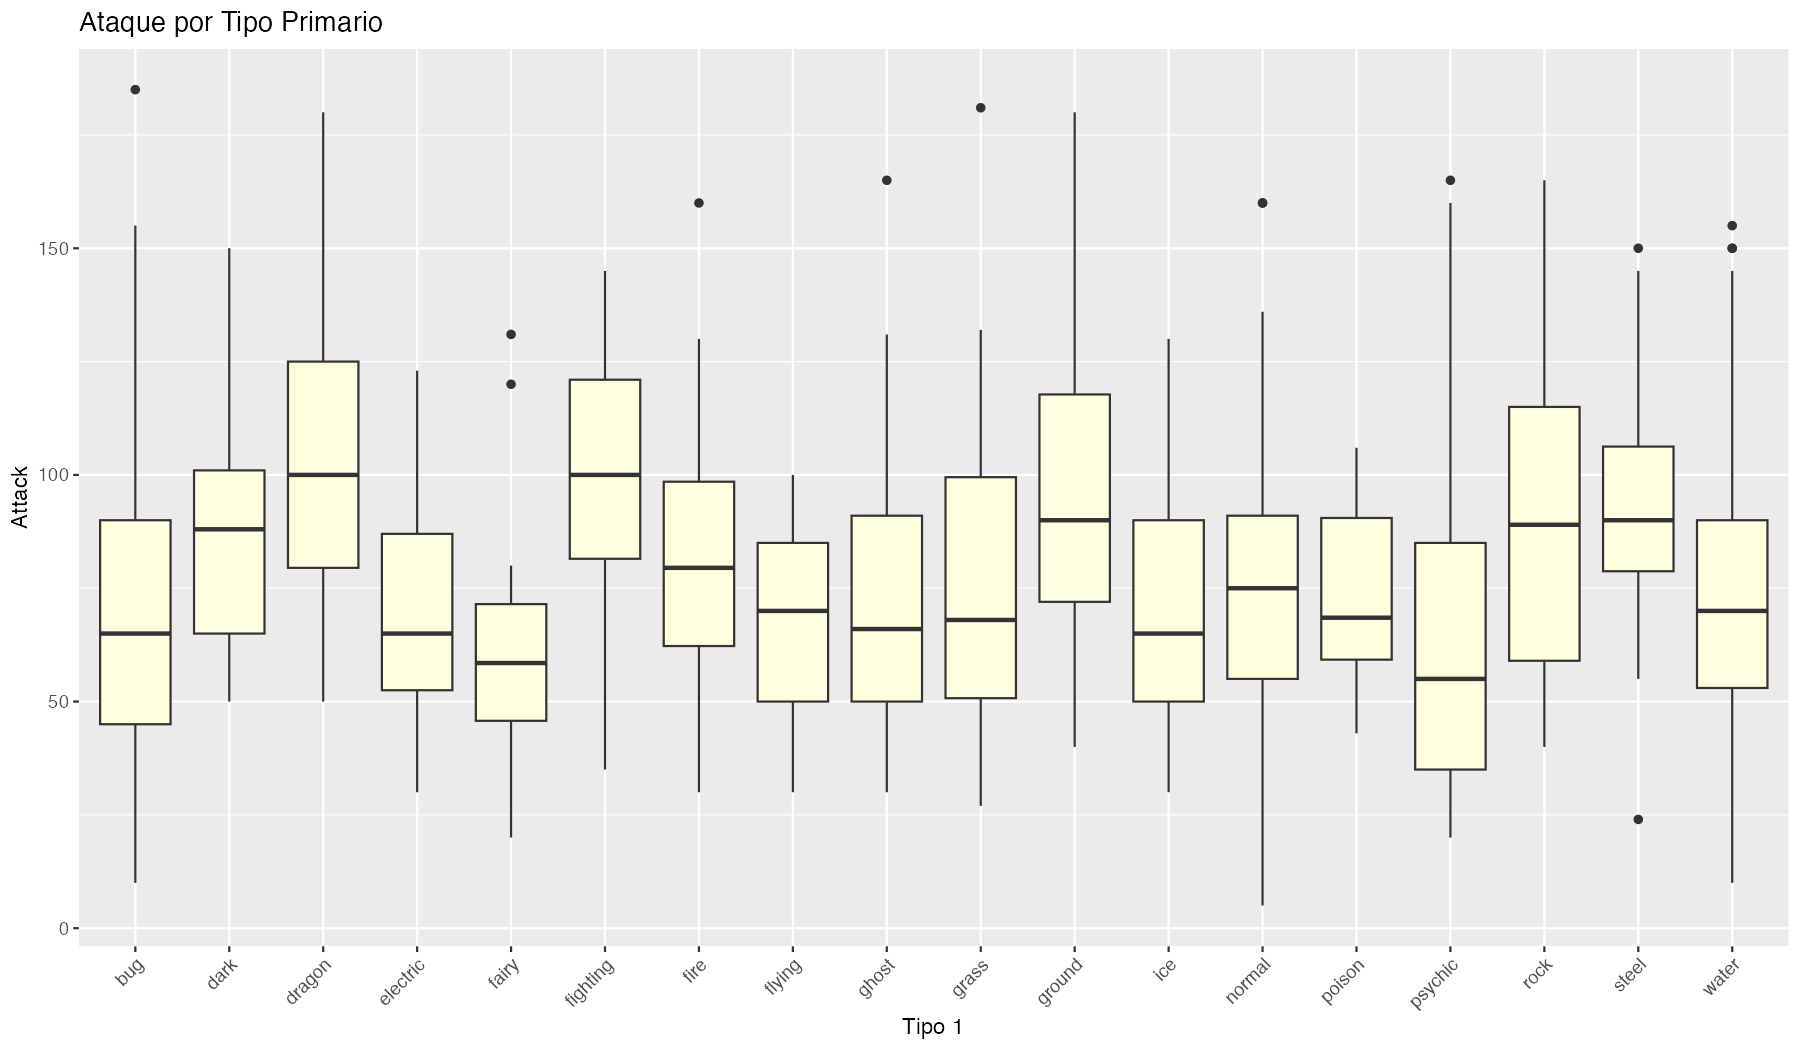
\includegraphics[width=\textwidth]{plots/box_attack_type1.png}
  \caption{Distribución del ataque (attack) por tipo primario (type1).}
\end{figure}

\textbf{Boxplot: Attack vs Generation}

Los valores de ataque son relativamente similares entre generaciones, aunque la generación 4 y 7
muestran medianas ligeramente superiores. Se aprecian varios valores atípicos en todas las generaciones.

\begin{lstlisting}[style=Rstyle]
ggplot(pokemon, aes(x = generation, y = attack)) +
  geom_boxplot(fill = "lightblue") +
  labs(title = "Ataque por Generacion", x = "Generacion", y = "Attack")
\end{lstlisting}

\begin{figure}[H]
  \centering
  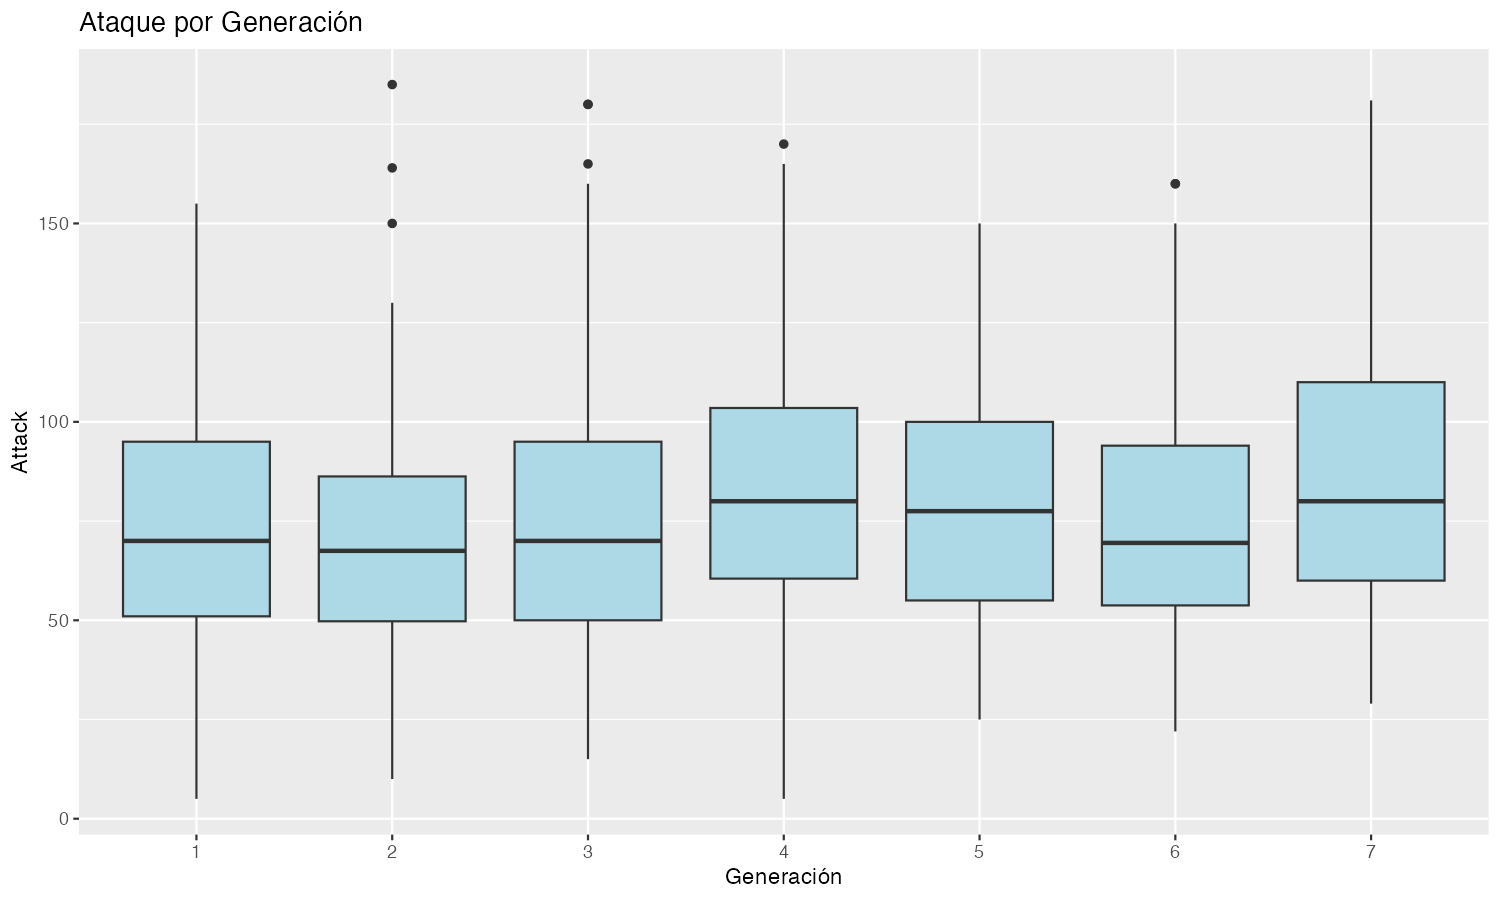
\includegraphics[width=0.85\textwidth]{plots/box_attack_generation.png}
  \caption{Distribución del ataque por generación.}
\end{figure}

\textbf{Boxplot: Defense vs Type1}

Los Pokémon de tipo \textbf{steel} (acero) presentan la mayor mediana de defensa, seguidos de
\textbf{rock} (roca) y \textbf{ground} (tierra). Los tipos \textbf{normal} y \textbf{psychic}
muestran las defensas más bajas en promedio.

\begin{lstlisting}[style=Rstyle]
ggplot(pokemon, aes(x = type1, y = defense)) +
  geom_boxplot(fill = "lightgreen") +
  theme(axis.text.x = element_text(angle = 45, hjust = 1)) +
  labs(title = "Defensa por Tipo Primario", x = "Tipo 1", y = "Defense")
\end{lstlisting}

\begin{figure}[H]
  \centering
  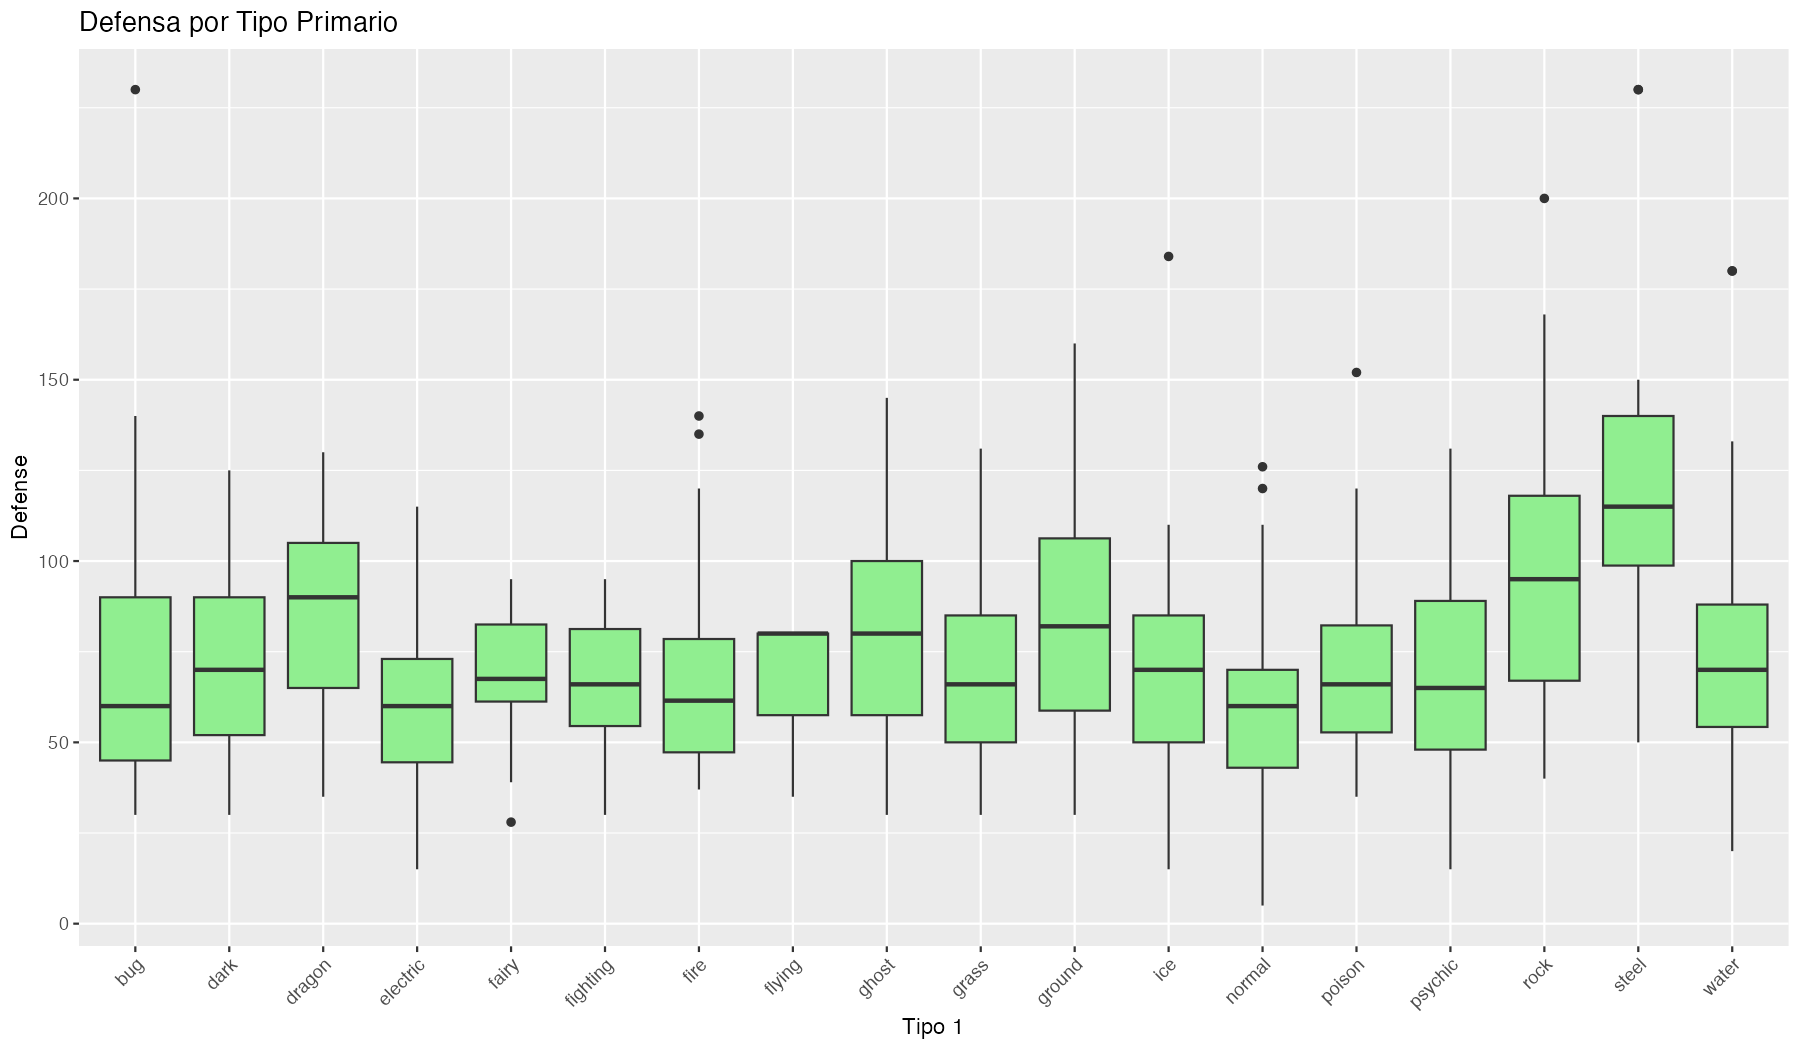
\includegraphics[width=\textwidth]{plots/box_defense_type1.png}
  \caption{Distribución de la defensa (defense) por tipo primario (type1).}
\end{figure}

\textbf{Boxplot: Attack vs Type2}

Al analizar el ataque según el tipo secundario, se observa que Pokémon con tipo 2 \textbf{rock}
(roca) y \textbf{dragon} presentan altos valores de ataque. Los Pokémon sin tipo secundario (categoría
vacía) tienen una amplia dispersión.

\begin{lstlisting}[style=Rstyle]
ggplot(pokemon, aes(x = type2, y = attack)) +
  geom_boxplot(fill = "lightsalmon") +
  theme(axis.text.x = element_text(angle = 45, hjust = 1)) +
  labs(title = "Ataque por Tipo Secundario", x = "Tipo 2", y = "Attack")
\end{lstlisting}

\begin{figure}[H]
  \centering
  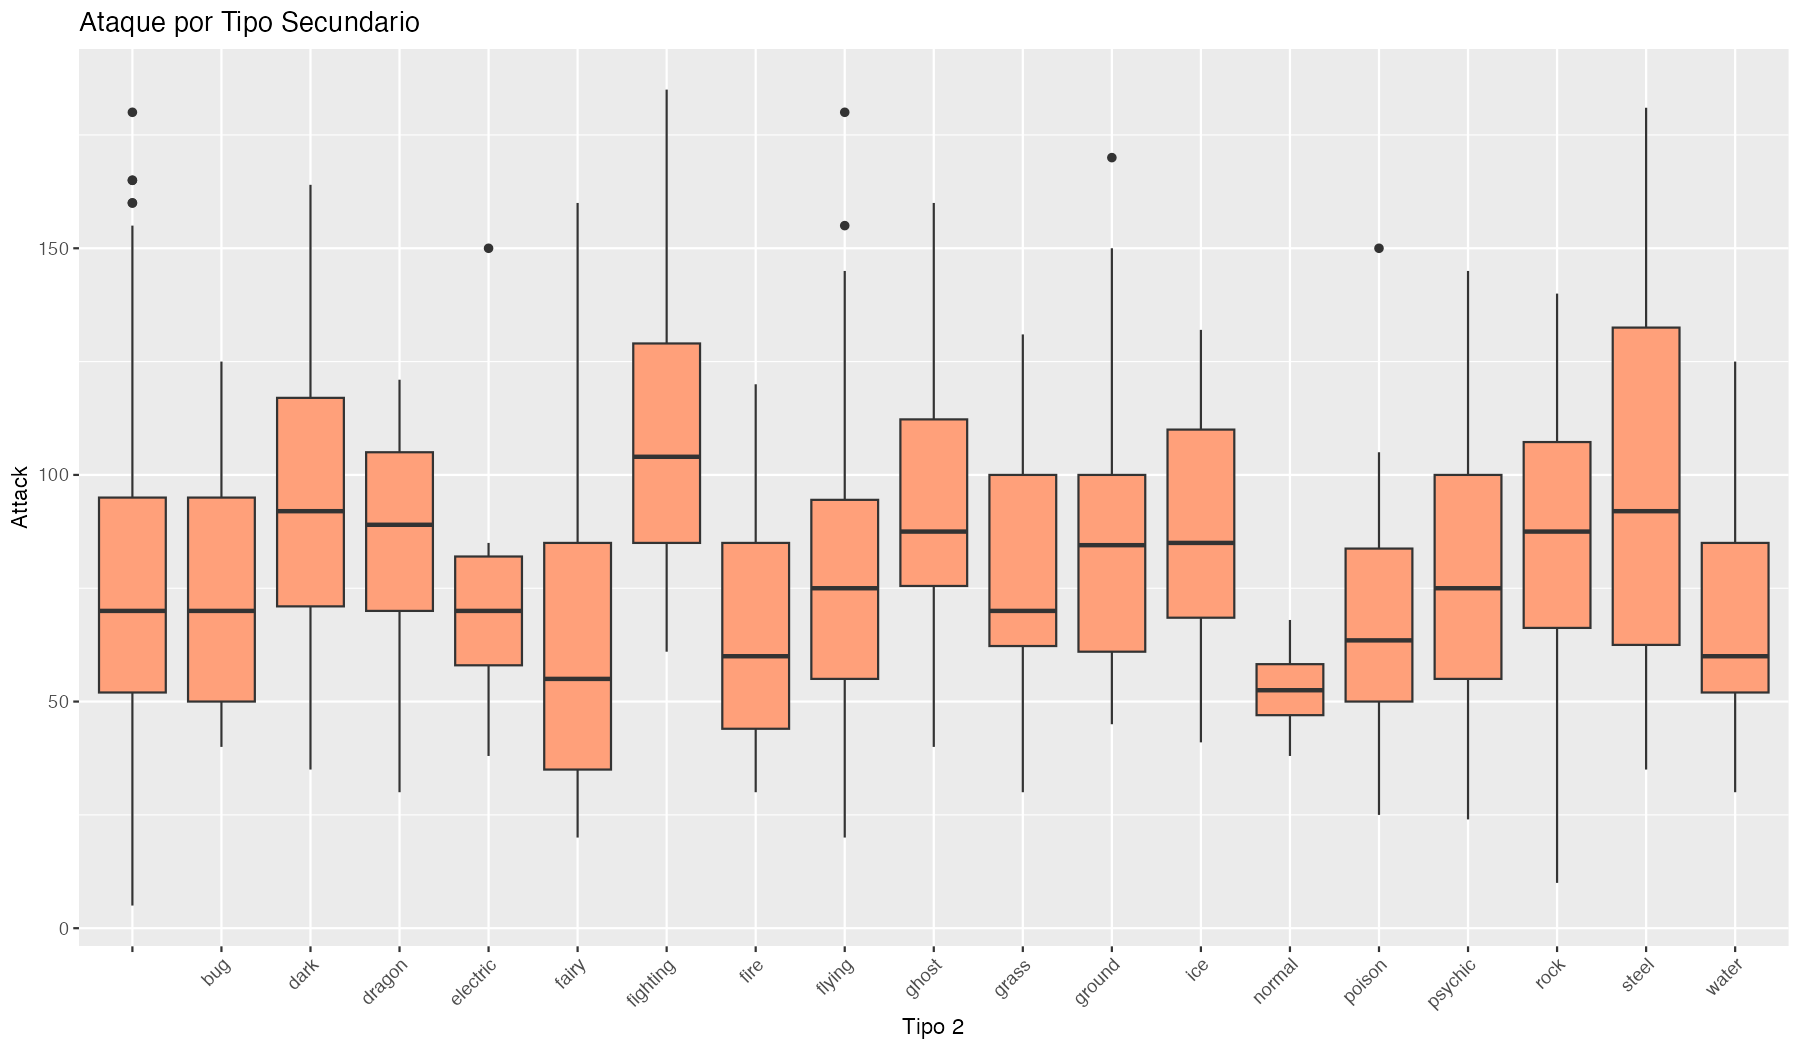
\includegraphics[width=\textwidth]{plots/box_attack_type2.png}
  \caption{Distribución del ataque (attack) por tipo secundario (type2).}
\end{figure}

\textbf{Boxplot: HP vs Type1}

Los Pokémon de tipo \textbf{normal} y \textbf{dragon} tienen las medianas de HP más altas.
Los tipos \textbf{ghost} y \textbf{fighting} presentan medianas de HP más bajas.

\begin{lstlisting}[style=Rstyle]
ggplot(pokemon, aes(x = type1, y = hp)) +
  geom_boxplot(fill = "plum") +
  theme(axis.text.x = element_text(angle = 45, hjust = 1)) +
  labs(title = "HP por Tipo Primario", x = "Tipo 1", y = "HP")
\end{lstlisting}

\begin{figure}[H]
  \centering
  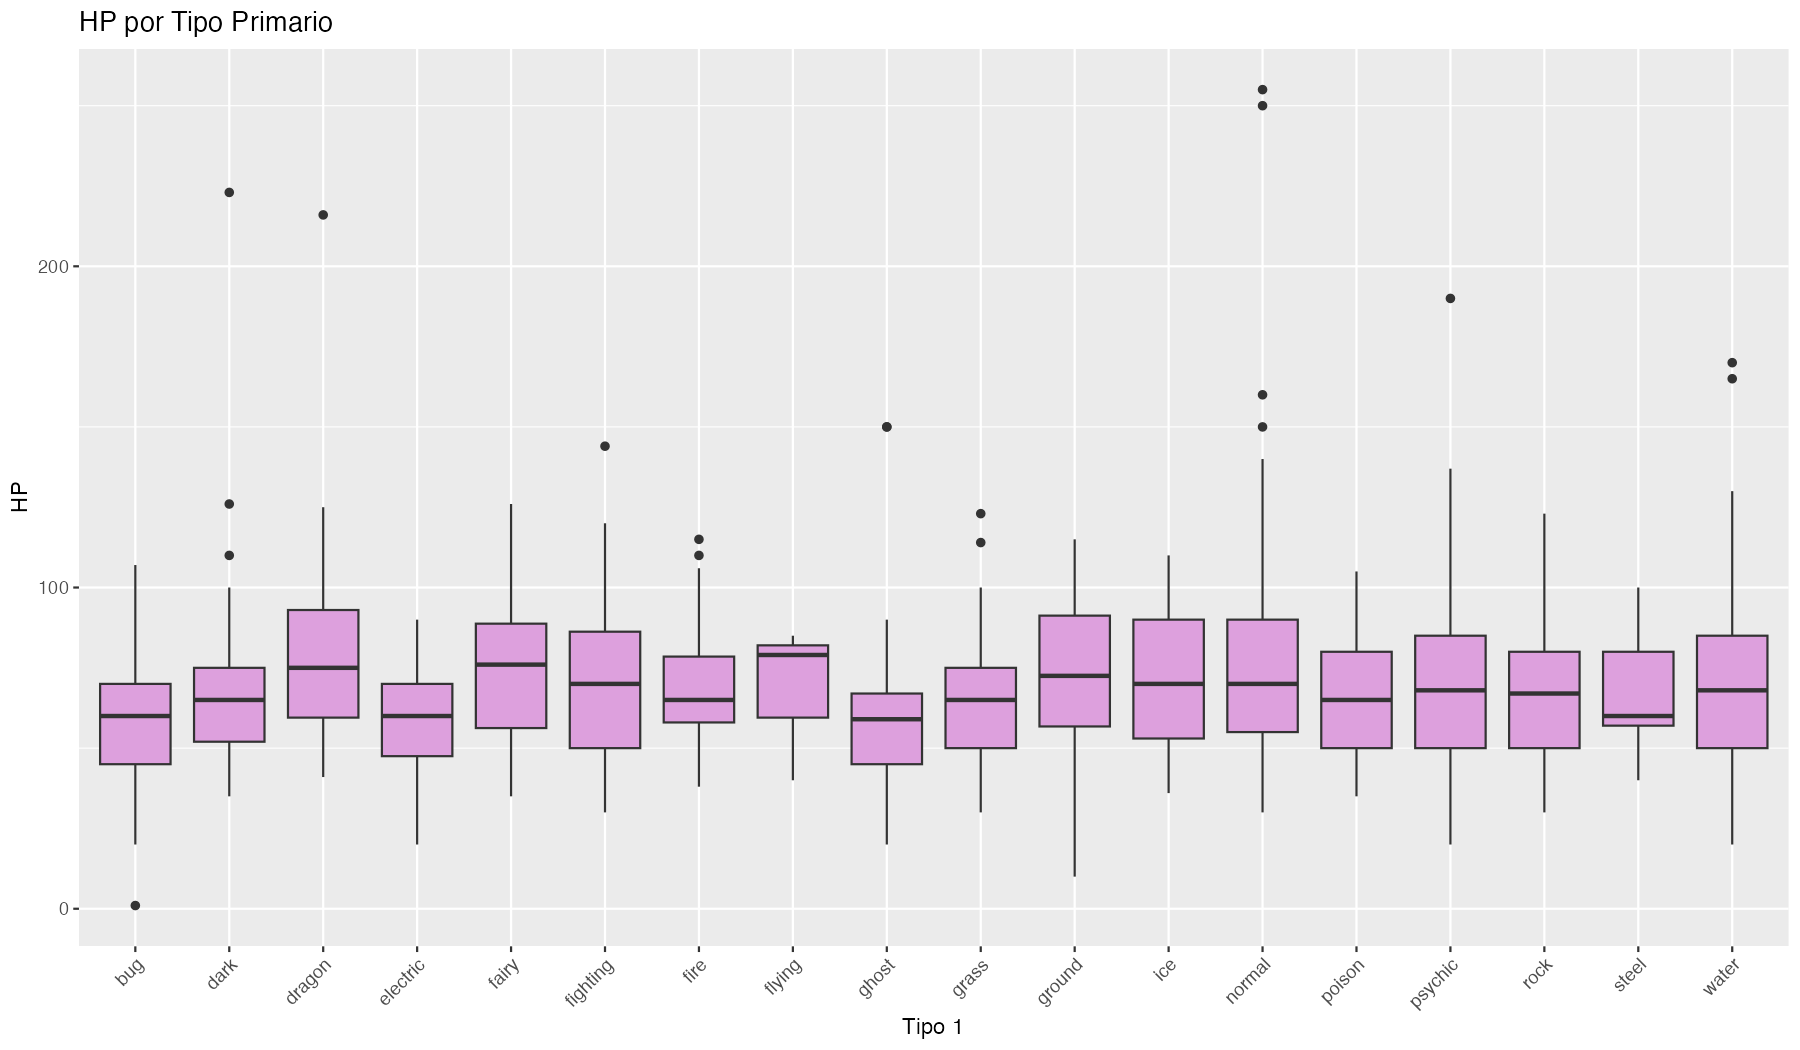
\includegraphics[width=\textwidth]{plots/box_hp_type1.png}
  \caption{Distribución de HP (puntos de vida) por tipo primario (type1).}
\end{figure}

% ============================================================
\subsection{A.5 Polígonos de Frecuencia}

Los polígonos de frecuencia son una alternativa a los histogramas para comparar la distribución
de una variable continua entre varios grupos categóricos, usando líneas en lugar de barras.

\textbf{Polígono de frecuencia: Attack vs is\_legendary}

El siguiente gráfico es el provisto en el enunciado. Se puede observar que los Pokémon no
legendarios (0) concentran sus valores de ataque alrededor de 50--75, mientras que los
legendarios (1) muestran una distribución más dispersa con mayor presencia en valores altos.

\begin{lstlisting}[style=Rstyle]
ggplot(pokemon, aes(x = attack, color = is_legendary)) +
  geom_freqpoly(binwidth = 10)
\end{lstlisting}

\begin{figure}[H]
  \centering
  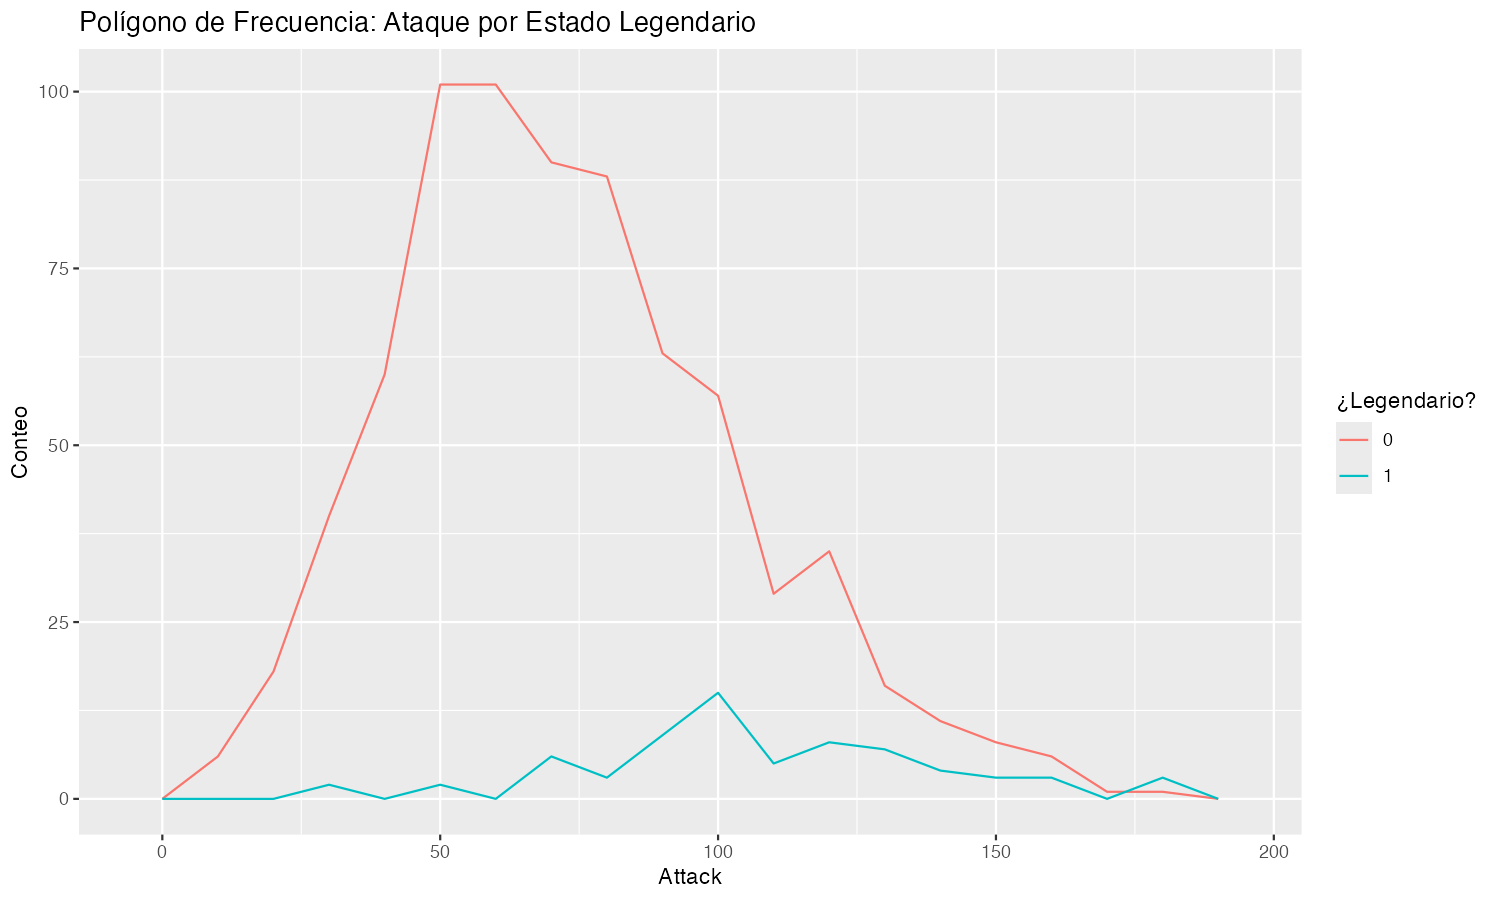
\includegraphics[width=0.9\textwidth]{plots/freqpoly_attack_legendary.png}
  \caption{Polígono de frecuencia del ataque (attack) comparando Pokémon legendarios (1) y no legendarios (0).}
\end{figure}

\textbf{Polígono de frecuencia: Defense vs Generation}

Las generaciones presentan distribuciones de defensa muy similares entre sí, con mayor concentración
de valores bajos (entre 40 y 80) en todas las generaciones.

\begin{lstlisting}[style=Rstyle]
ggplot(pokemon, aes(x = defense, color = generation)) +
  geom_freqpoly(binwidth = 10) +
  labs(title = "Poligono de Frecuencia: Defensa por Generacion",
       x = "Defense", y = "Conteo", color = "Generacion")
\end{lstlisting}

\begin{figure}[H]
  \centering
  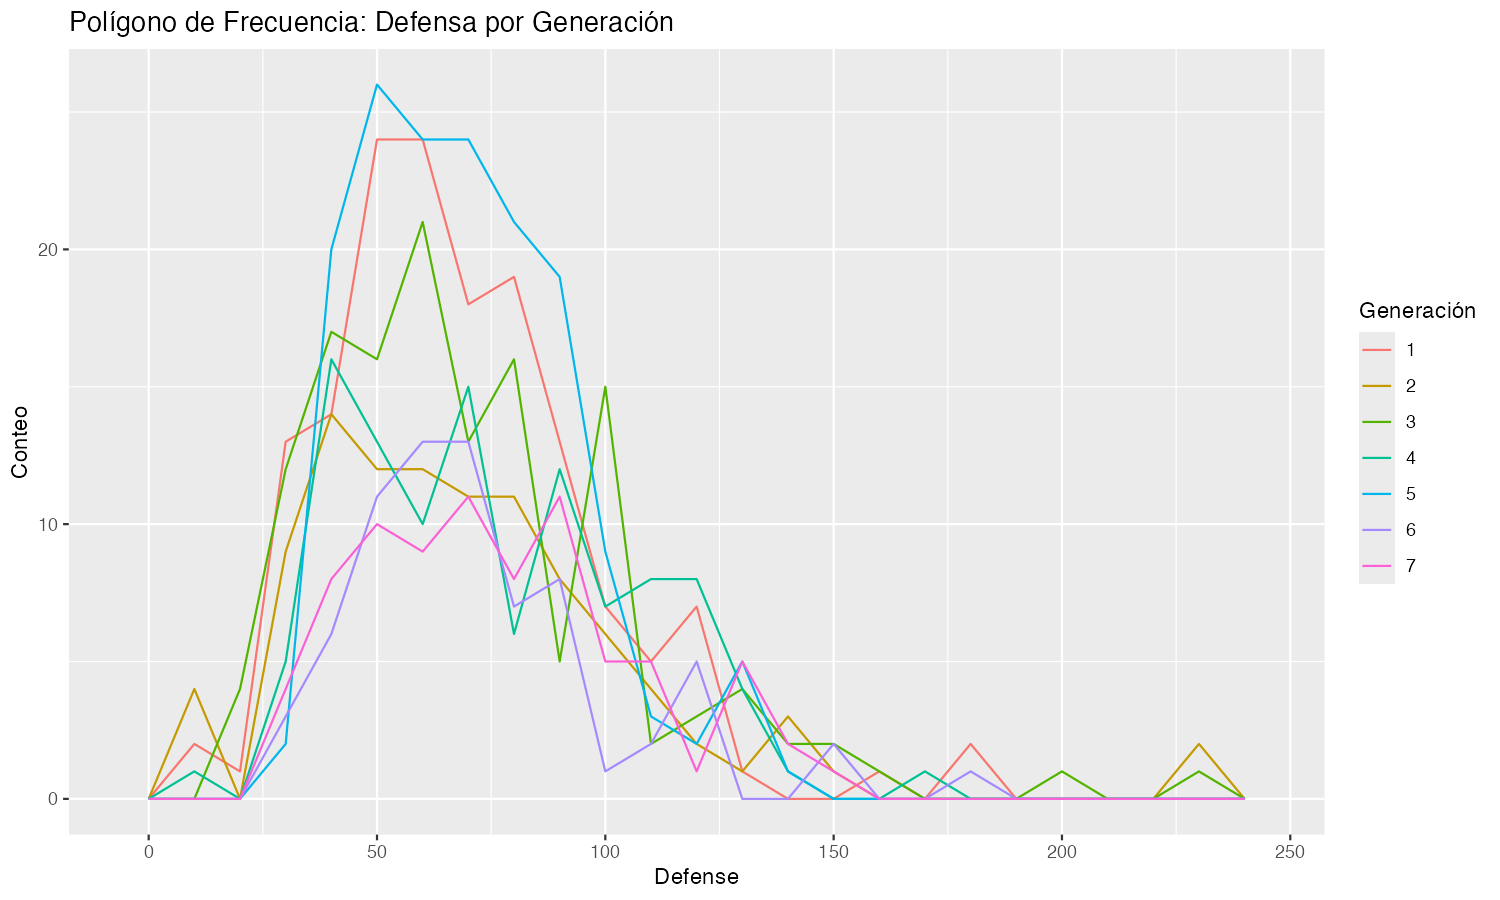
\includegraphics[width=0.9\textwidth]{plots/freqpoly_defense_generation.png}
  \caption{Polígono de frecuencia de la defensa (defense) por generación.}
\end{figure}

\textbf{Polígono de frecuencia: HP vs Generation}

Las distribuciones de HP por generación son muy similares, todas centradas alrededor de 50--70 HP.
No se aprecia una diferencia sistemática entre generaciones en cuanto a esta característica.

\begin{lstlisting}[style=Rstyle]
ggplot(pokemon, aes(x = hp, color = generation)) +
  geom_freqpoly(binwidth = 10) +
  labs(title = "Poligono de Frecuencia: HP por Generacion",
       x = "HP", y = "Conteo", color = "Generacion")
\end{lstlisting}

\begin{figure}[H]
  \centering
  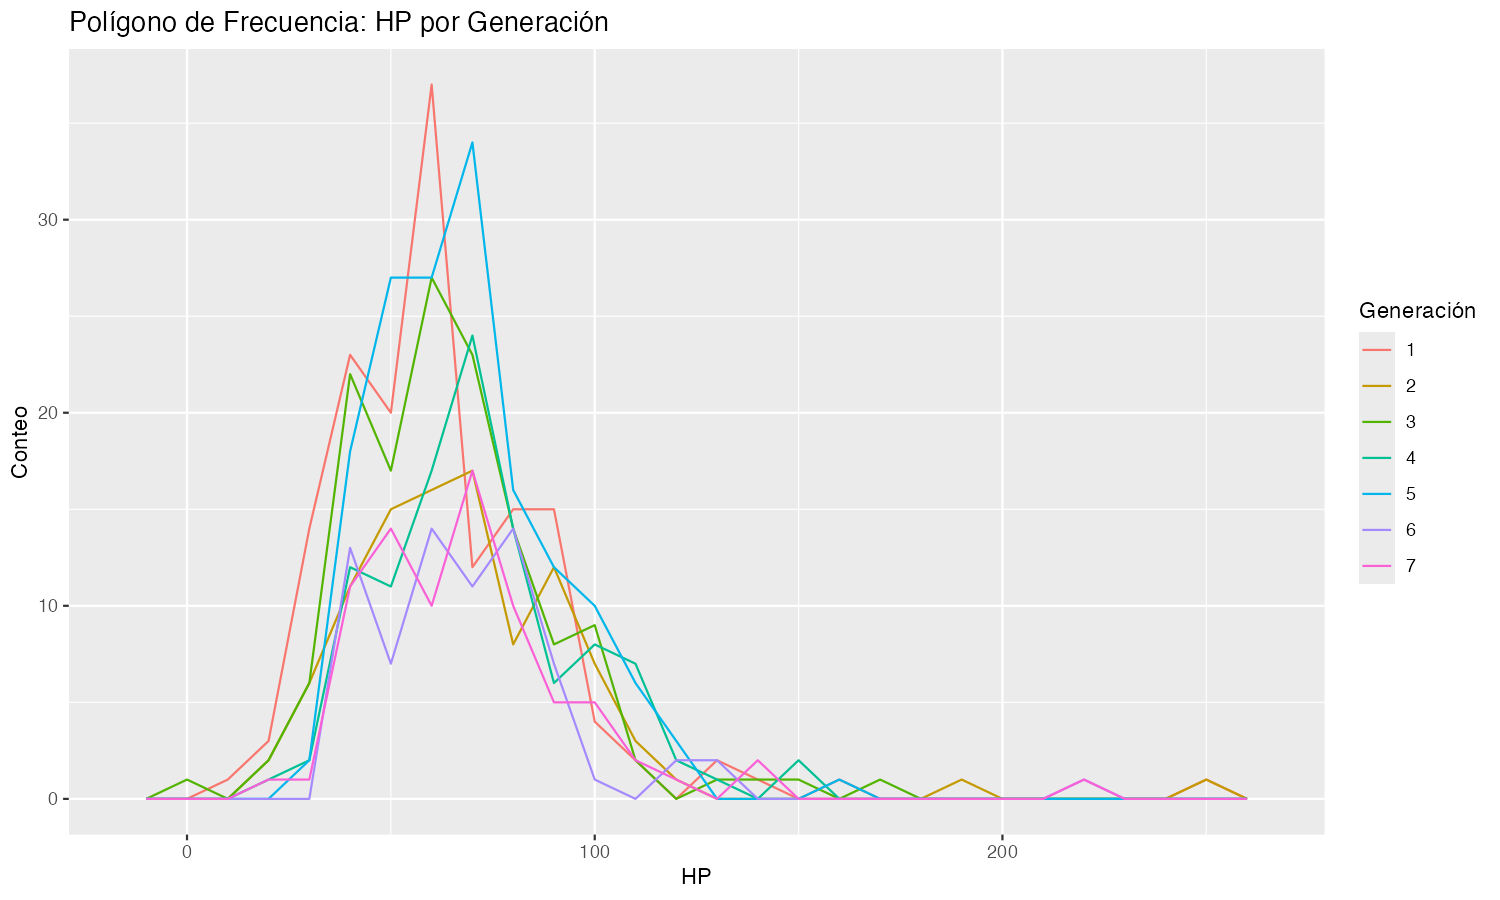
\includegraphics[width=0.9\textwidth]{plots/freqpoly_hp_generation.png}
  \caption{Polígono de frecuencia del HP por generación.}
\end{figure}

\textbf{Polígono de frecuencia: Weight\_kg vs is\_legendary}

La distribución de peso muestra que los Pokémon no legendarios se concentran fuertemente en
pesos bajos (menos de 100 kg), mientras que los legendarios presentan una distribución más
uniforme y extendida hacia pesos mayores.

\begin{lstlisting}[style=Rstyle]
ggplot(pokemon, aes(x = weight_kg, color = is_legendary)) +
  geom_freqpoly(binwidth = 20) +
  labs(title = "Poligono de Frecuencia: Peso por Estado Legendario",
       x = "Weight (kg)", y = "Conteo", color = "Legendario")
\end{lstlisting}

\begin{figure}[H]
  \centering
  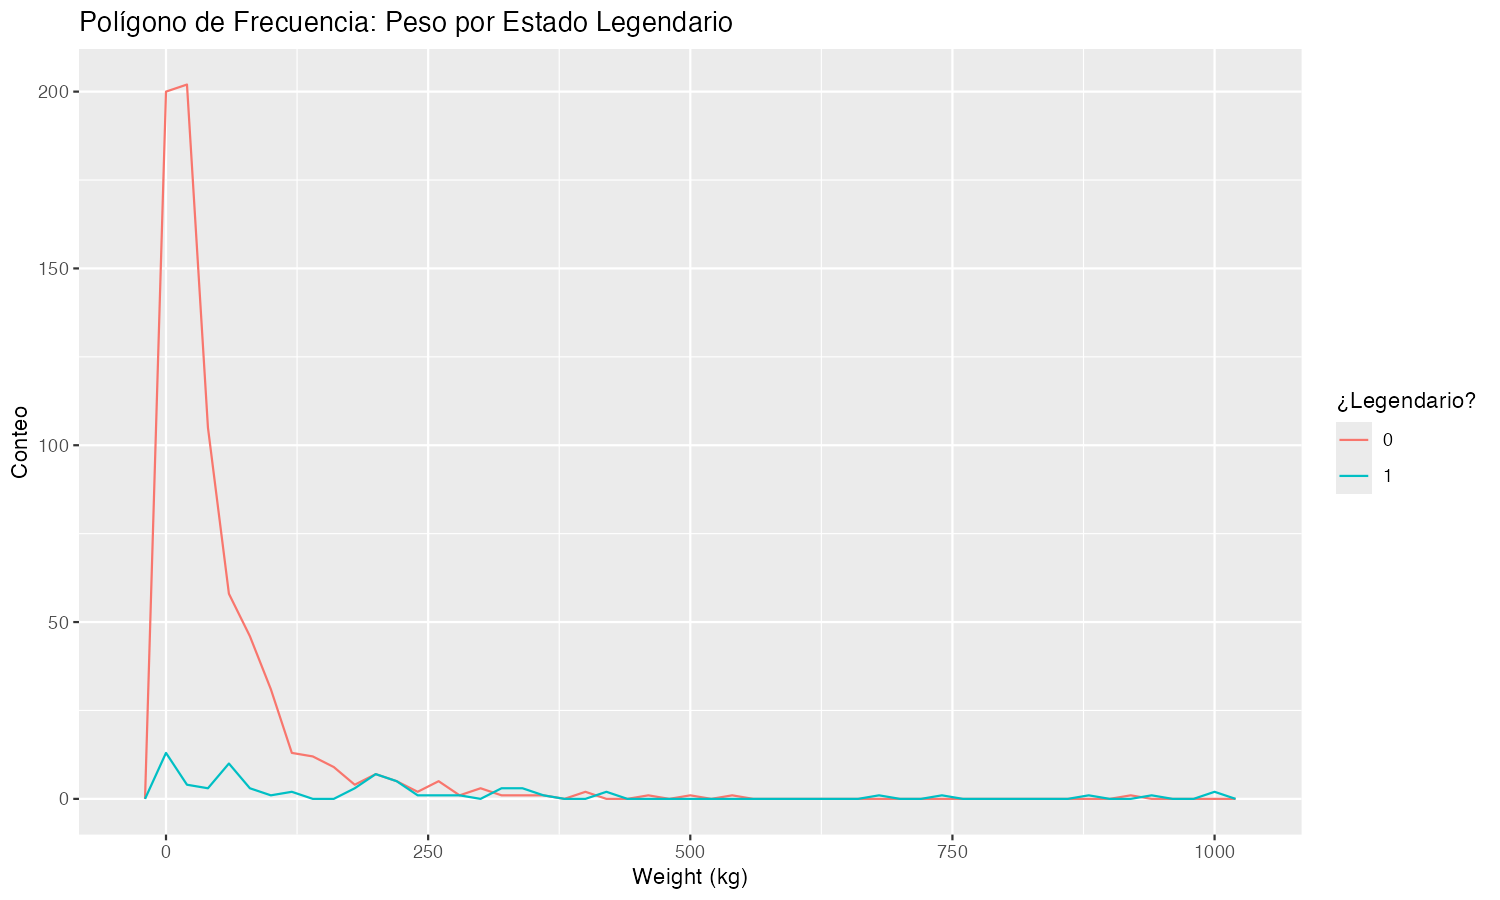
\includegraphics[width=0.9\textwidth]{plots/freqpoly_weight_legendary.png}
  \caption{Polígono de frecuencia del peso (weight\_kg) según estado legendario.}
\end{figure}

% ============================================================
\subsection{A.6 Gráficos de Dispersión}

Los diagramas de dispersión permiten explorar la relación entre dos variables continuas,
ayudando a identificar posibles correlaciones o patrones.

\textbf{Dispersión: Attack vs Defense}

El siguiente gráfico es el provisto en el enunciado. Se puede observar una ligera tendencia
positiva: Pokémon con alto ataque tienden a tener también una defensa moderada o alta,
aunque la correlación no es muy pronunciada.

\begin{lstlisting}[style=Rstyle]
ggplot(pokemon, aes(x = attack, y = defense)) +
  geom_point()
\end{lstlisting}

\begin{figure}[H]
  \centering
  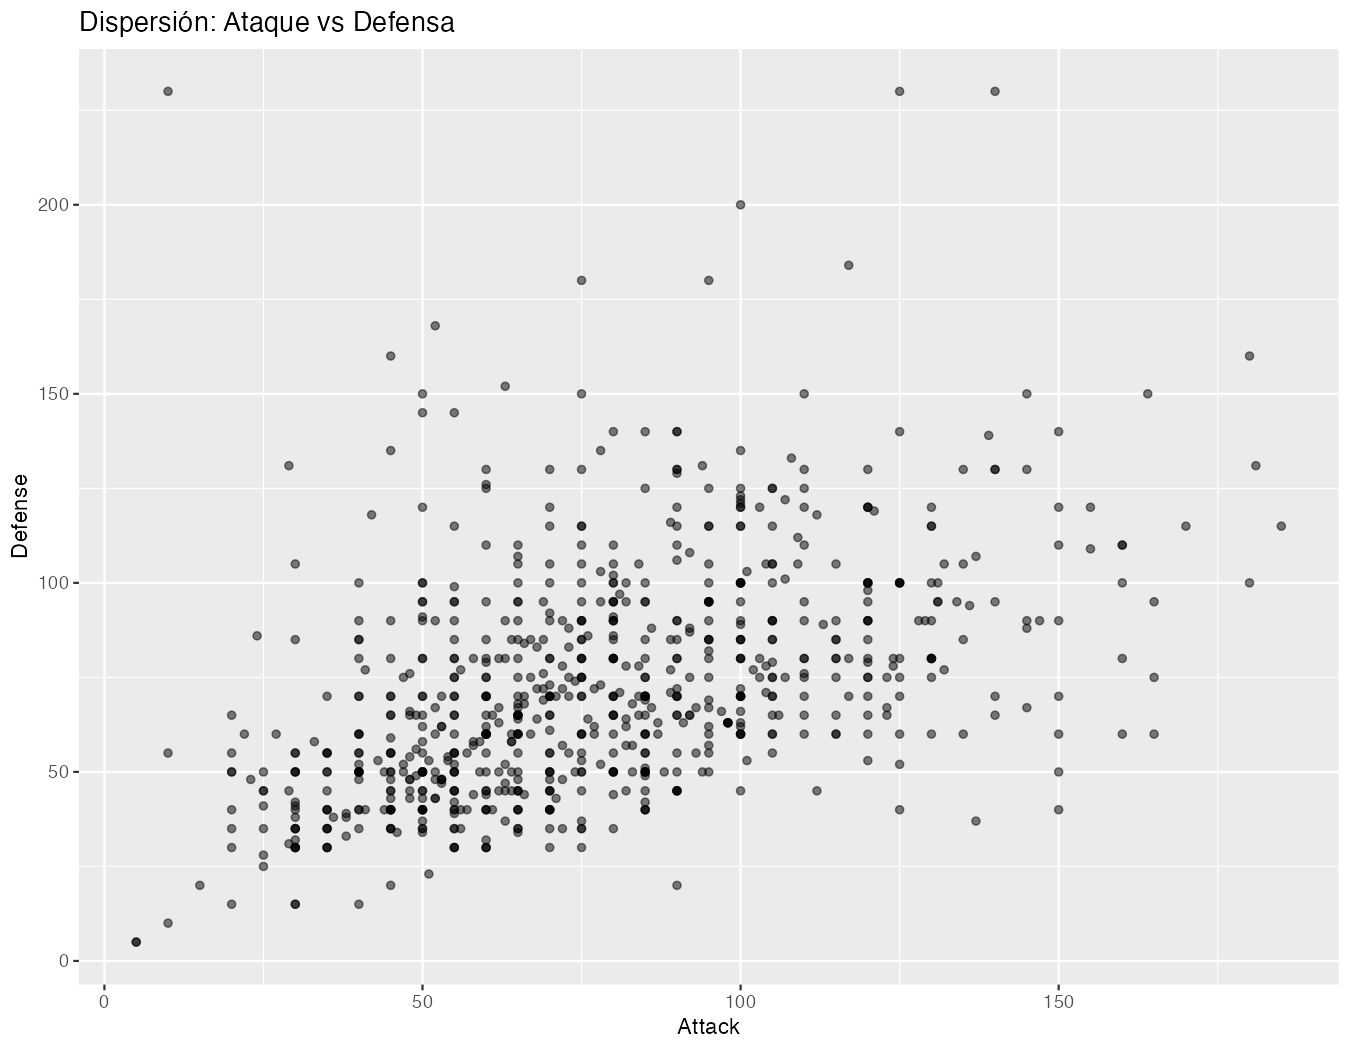
\includegraphics[width=0.85\textwidth]{plots/scatter_attack_defense.png}
  \caption{Diagrama de dispersión entre el ataque (attack) y la defensa (defense).}
\end{figure}

\textbf{Dispersión: Attack vs Speed}

No se aprecia una correlación clara entre ataque y velocidad; los puntos se distribuyen de forma
relativamente aleatoria, sugiriendo que ambas son estadísticas independientes en el diseño de los Pokémon.

\begin{lstlisting}[style=Rstyle]
ggplot(pokemon, aes(x = attack, y = speed)) +
  geom_point(alpha = 0.5, color = "steelblue") +
  labs(title = "Dispersion: Ataque vs Velocidad",
       x = "Attack", y = "Speed")
\end{lstlisting}

\begin{figure}[H]
  \centering
  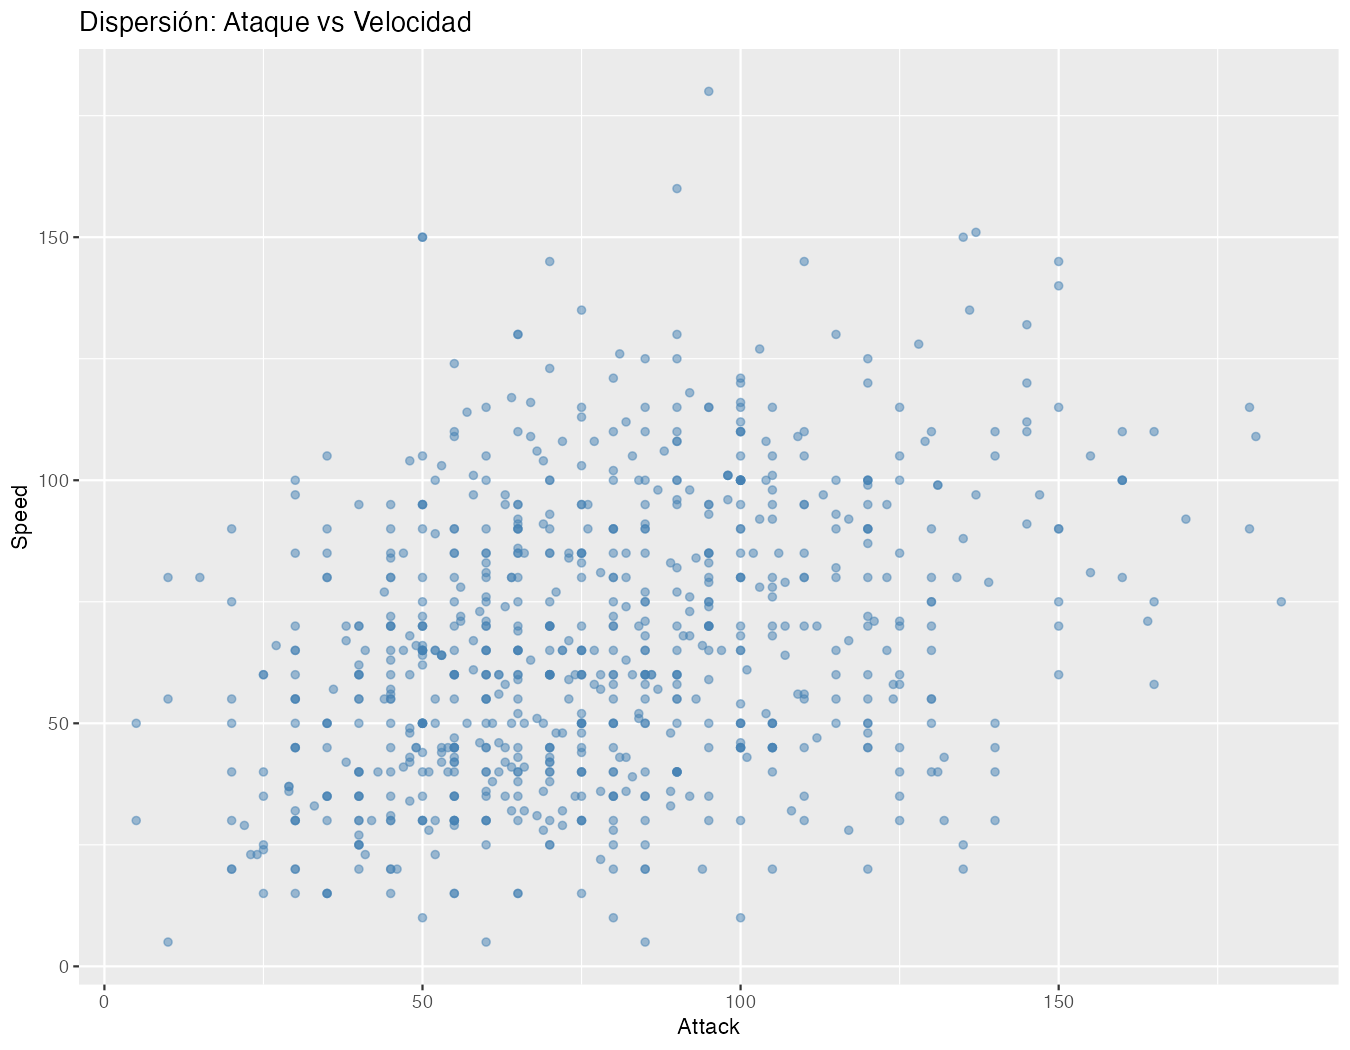
\includegraphics[width=0.85\textwidth]{plots/scatter_attack_speed.png}
  \caption{Diagrama de dispersión entre el ataque (attack) y la velocidad (speed).}
\end{figure}

\textbf{Dispersión: Speed vs Defense}

Existe una tendencia inversa débil entre velocidad y defensa: Pokémon muy veloces tienden a
tener defensas moderadas, mientras que los más lentos pueden tener defensas muy altas (e.g.,
tipo acero o roca).

\begin{lstlisting}[style=Rstyle]
ggplot(pokemon, aes(x = speed, y = defense)) +
  geom_point(alpha = 0.5, color = "tomato") +
  labs(title = "Dispersion: Velocidad vs Defensa",
       x = "Speed", y = "Defense")
\end{lstlisting}

\begin{figure}[H]
  \centering
  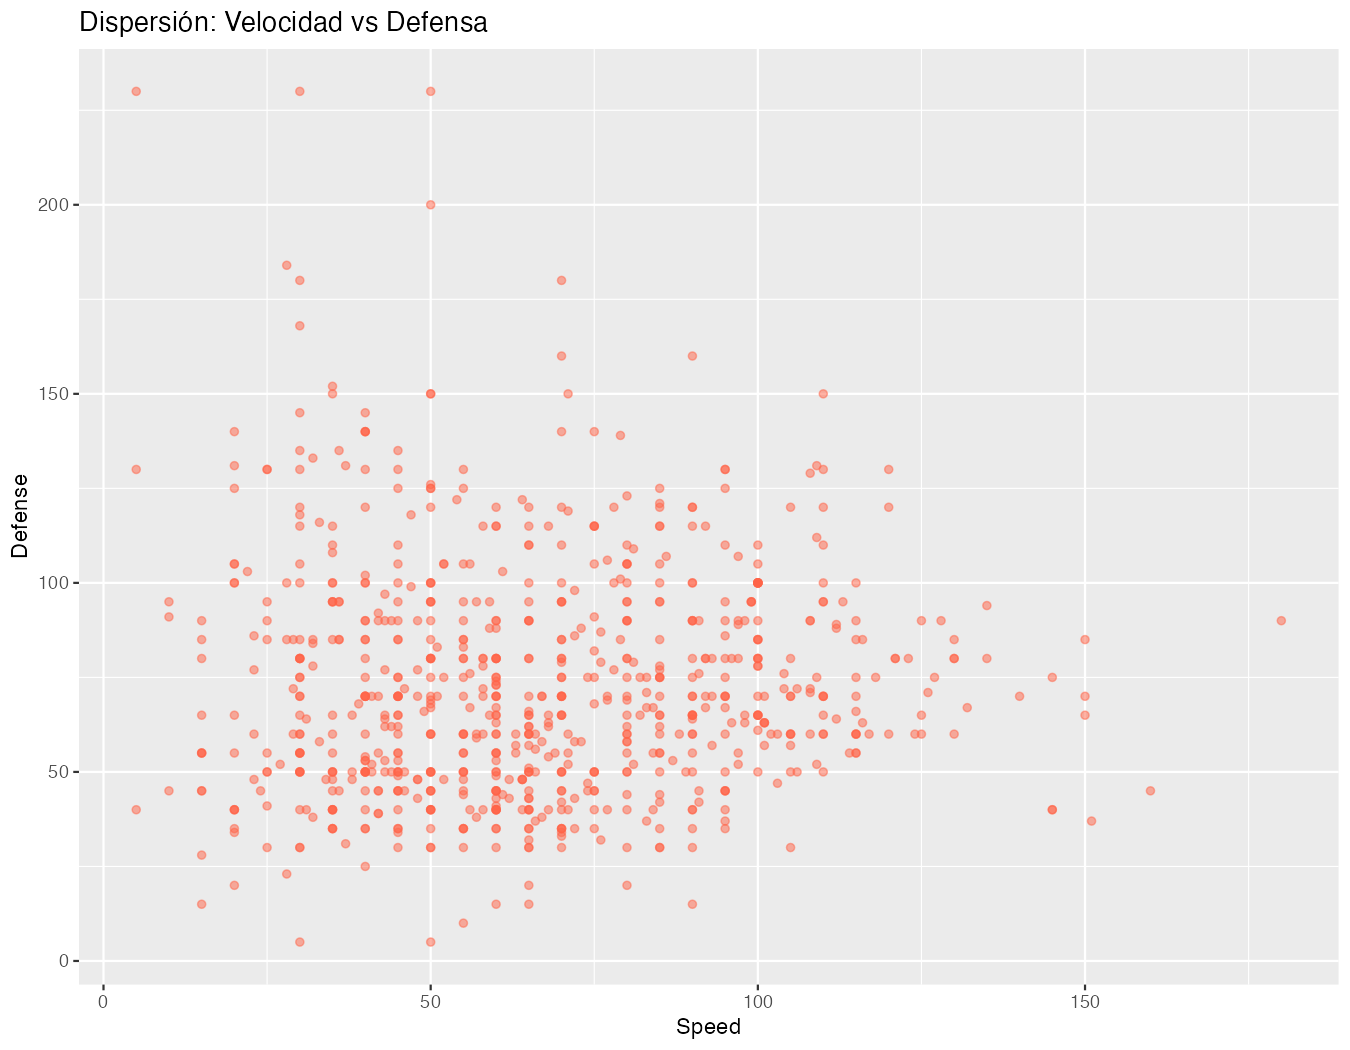
\includegraphics[width=0.85\textwidth]{plots/scatter_speed_defense.png}
  \caption{Diagrama de dispersión entre la velocidad (speed) y la defensa (defense).}
\end{figure}

\textbf{Dispersión: Speed vs HP}

No se observa una correlación clara entre velocidad y puntos de vida. Los valores de HP se
distribuyen de forma similar en todo el rango de velocidades.

\begin{lstlisting}[style=Rstyle]
ggplot(pokemon, aes(x = speed, y = hp)) +
  geom_point(alpha = 0.5, color = "mediumseagreen") +
  labs(title = "Dispersion: Velocidad vs HP",
       x = "Speed", y = "HP")
\end{lstlisting}

\begin{figure}[H]
  \centering
  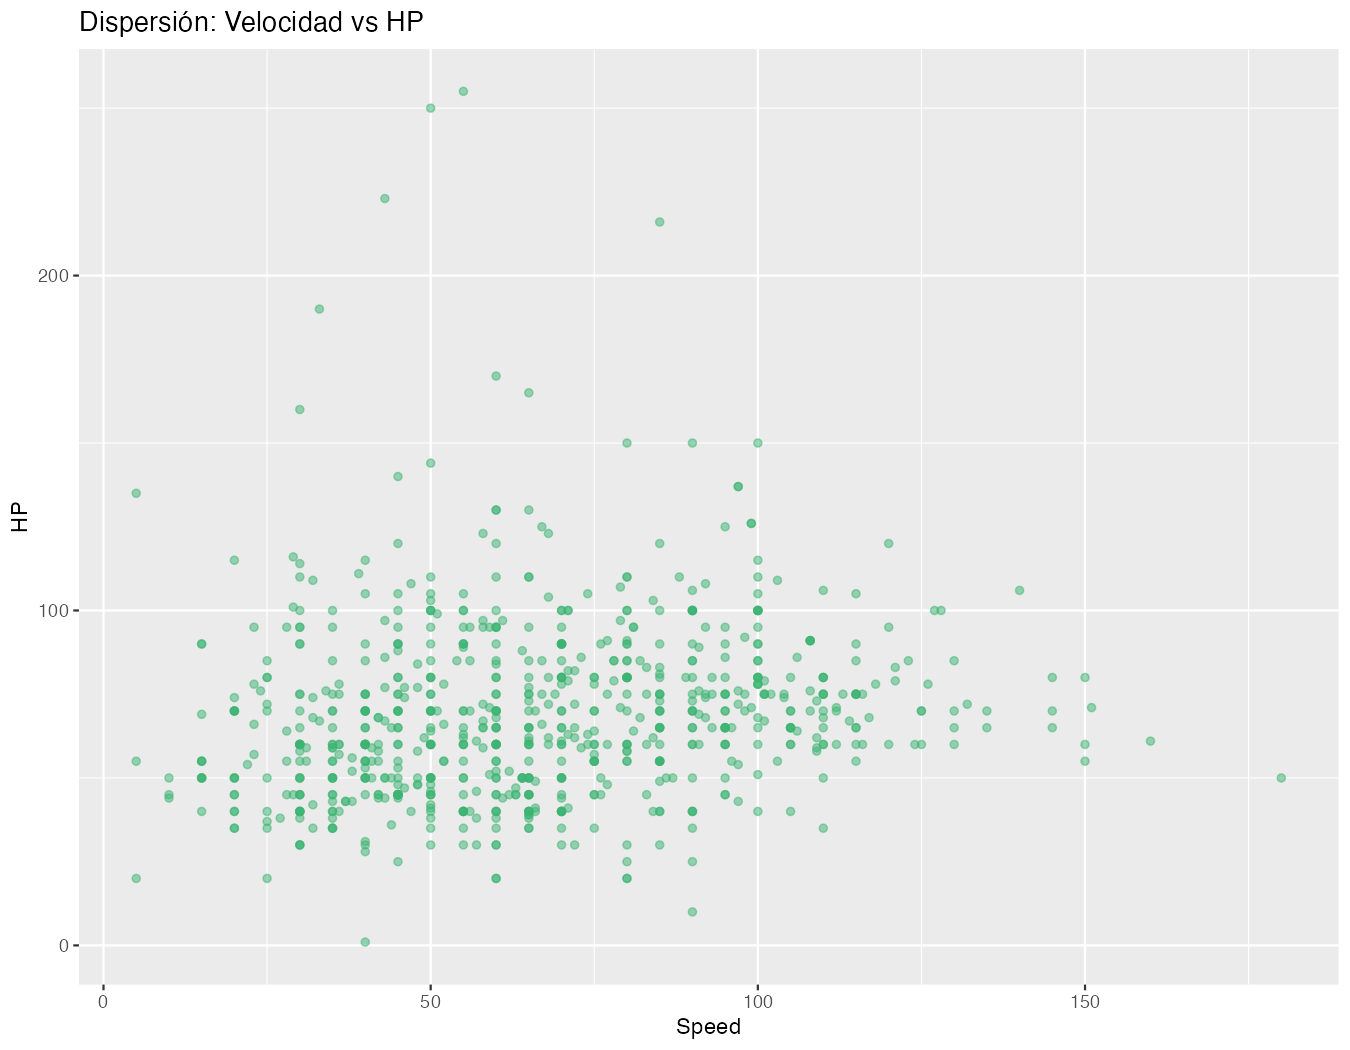
\includegraphics[width=0.85\textwidth]{plots/scatter_speed_hp.png}
  \caption{Diagrama de dispersión entre la velocidad (speed) y los puntos de vida (HP).}
\end{figure}

\textbf{Matriz de dispersión: HP, Attack, Speed}

La matriz de dispersión permite visualizar simultáneamente todas las combinaciones por pares
de tres o más variables. El código utilizado es el siguiente:

\begin{lstlisting}[style=Rstyle]
# Matrices de dispersion dos a dos para hp, attack y speed
pairs(df[, c("hp", "attack", "speed")], main = "Matrices de Dispersion")
\end{lstlisting}

\begin{figure}[H]
  \centering
  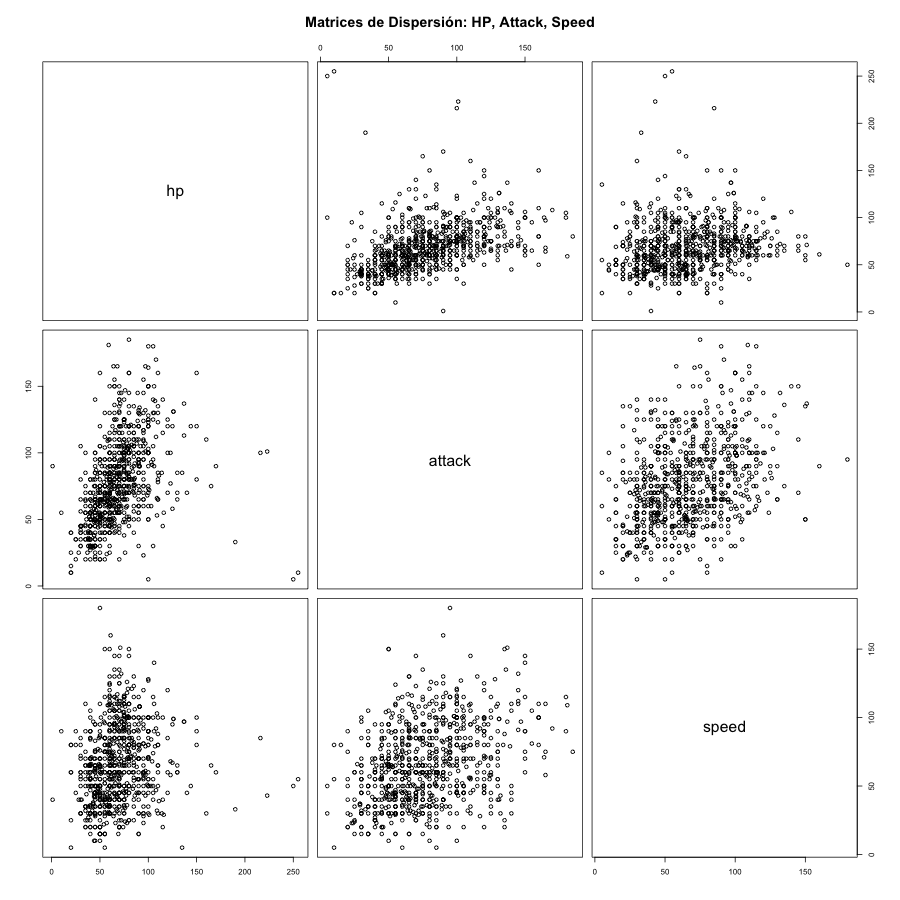
\includegraphics[width=0.85\textwidth]{plots/pairs_matrix.png}
  \caption{Matriz de dispersión para las variables HP, attack y speed.}
\end{figure}

La matriz muestra que ninguna de las tres variables presenta una correlación lineal fuerte entre sí,
confirmando que el diseño de los Pokémon tiende a distribuir estas estadísticas de forma independiente.

% ============================================================
\section{Parte B: Gráficos Depurados}
% ============================================================

En esta segunda parte se utilizan librerías adicionales para generar visualizaciones más elaboradas
y con mejor calidad visual. Se instalan y cargan los siguientes paquetes:

\begin{lstlisting}[style=Rstyle]
install.packages(c("dplyr", "ggplot2", "gridExtra", "tidyr",
                   "reshape2", "RColorBrewer", "ggrepel"))

library(dplyr)
library(ggplot2)
library(gridExtra)
library(tidyr)
library(reshape2)
library(RColorBrewer)
library(ggrepel)
\end{lstlisting}

Se convierte el data frame a formato \texttt{tibble} (un data frame simplificado con mejores
funcionalidades de impresión), se corrige el nombre de la columna 25 (\texttt{classfication}
a \texttt{classification}) y se convierte \texttt{capture\_rate} a numérico:

\begin{lstlisting}[style=Rstyle]
df <- tibble::as_tibble(df)
colnames(df)[25] <- "classification"
df$capture_rate <- as.numeric(df$capture_rate)
\end{lstlisting}

Dado que el data frame original es extenso, se seleccionan solo las columnas relevantes para
esta parte del laboratorio:

\begin{lstlisting}[style=Rstyle]
df <- select(df, name, classification, hp, weight_kg,
             height_m, speed, attack, defense,
             sp_attack, sp_defense, type1, type2,
             abilities, generation, is_legendary,
             capture_rate)
\end{lstlisting}

El resultado contiene las 16 columnas más relevantes para el análisis.

% ============================================================
\subsection{B.1 Gráficos de Densidad}

Un diagrama de densidad visualiza la distribución de datos en un intervalo continuo mediante el
suavizado del núcleo (kernel smoothing). A diferencia del histograma, produce curvas más suaves
que facilitan la identificación de la forma de la distribución y los picos de concentración de valores.

Se generó primero el grid original de 4 gráficos provisto en el enunciado:

\begin{lstlisting}[style=Rstyle]
density_hp <- ggplot(data=df, aes(hp)) +
  geom_density(col="white", fill="brown", alpha=0.8) +
  ggtitle("Densidad de Hit Points o Vida")

density_speed <- ggplot(data=df, aes(speed)) +
  geom_density(col="white", fill="blue", alpha=0.8) +
  ggtitle("Densidad de Velocidad")

density_attack <- ggplot(data=df, aes(attack)) +
  geom_density(col="white", fill="orange", alpha=0.7) +
  ggtitle("Densidad Caracteristicas Ofensivas")

density_defense <- ggplot(data=df, aes(defense)) +
  geom_density(col="white", fill="yellow", alpha=0.7) +
  ggtitle("Densidad Caracteristicas Defensivas")

grid.arrange(density_speed, density_hp, density_attack, density_defense, ncol=2)
\end{lstlisting}

\begin{figure}[H]
  \centering
  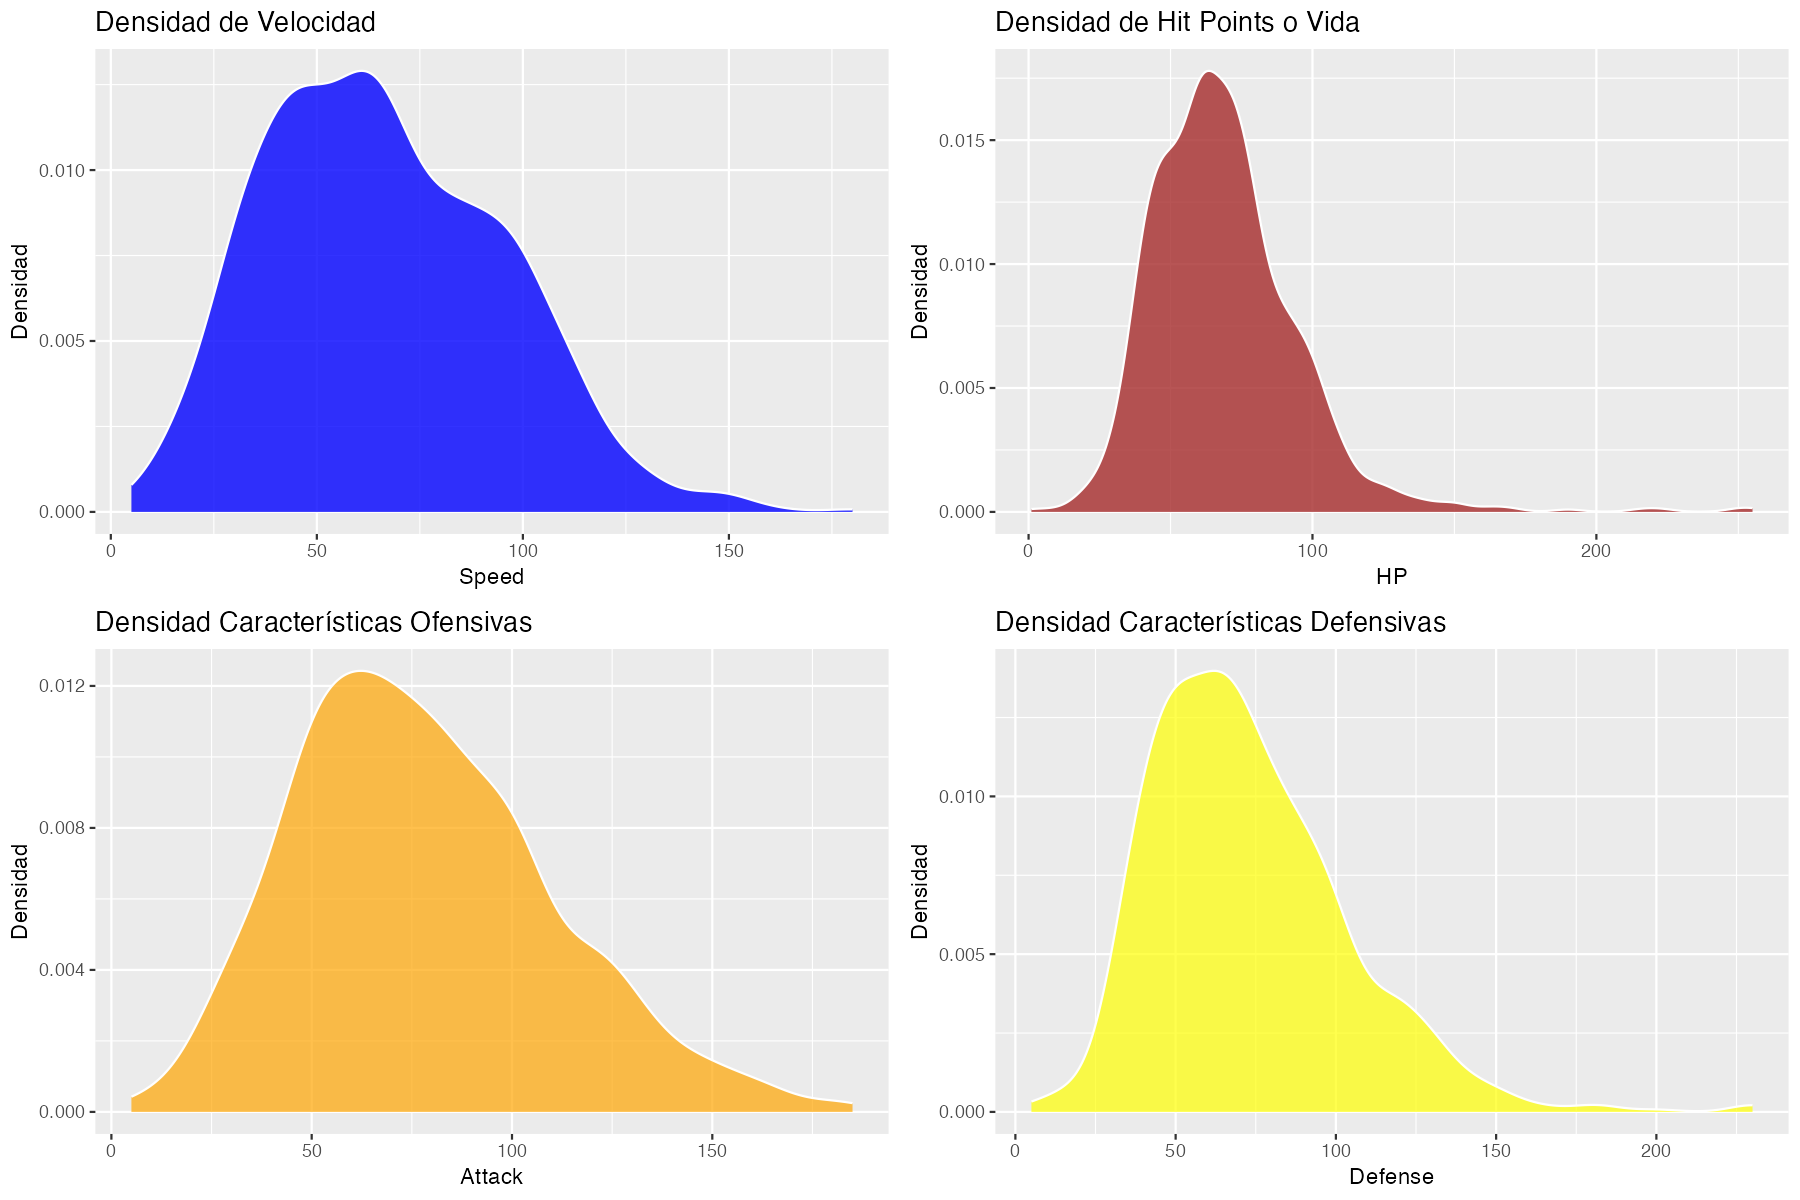
\includegraphics[width=\textwidth]{plots/density_grid_4.png}
  \caption{Grid de densidades de velocidad, HP, ataque y defensa de los Pokémon.}
\end{figure}

\textbf{Grid extendido (6 gráficos)}

Se amplía el grid anterior agregando los diagramas de densidad para \texttt{height\_m} y
\texttt{weight\_kg}, ahora organizado en 3 columnas:

\begin{lstlisting}[style=Rstyle]
density_height <- ggplot(data=df, aes(height_m)) +
  geom_density(col="white", fill="darkgreen", alpha=0.8) +
  ggtitle("Densidad de Altura (m)")

density_weight <- ggplot(data=df, aes(weight_kg)) +
  geom_density(col="white", fill="purple", alpha=0.8) +
  ggtitle("Densidad de Peso (kg)")

grid.arrange(density_speed, density_hp, density_attack,
             density_defense, density_height, density_weight, ncol=3)
\end{lstlisting}

\begin{figure}[H]
  \centering
  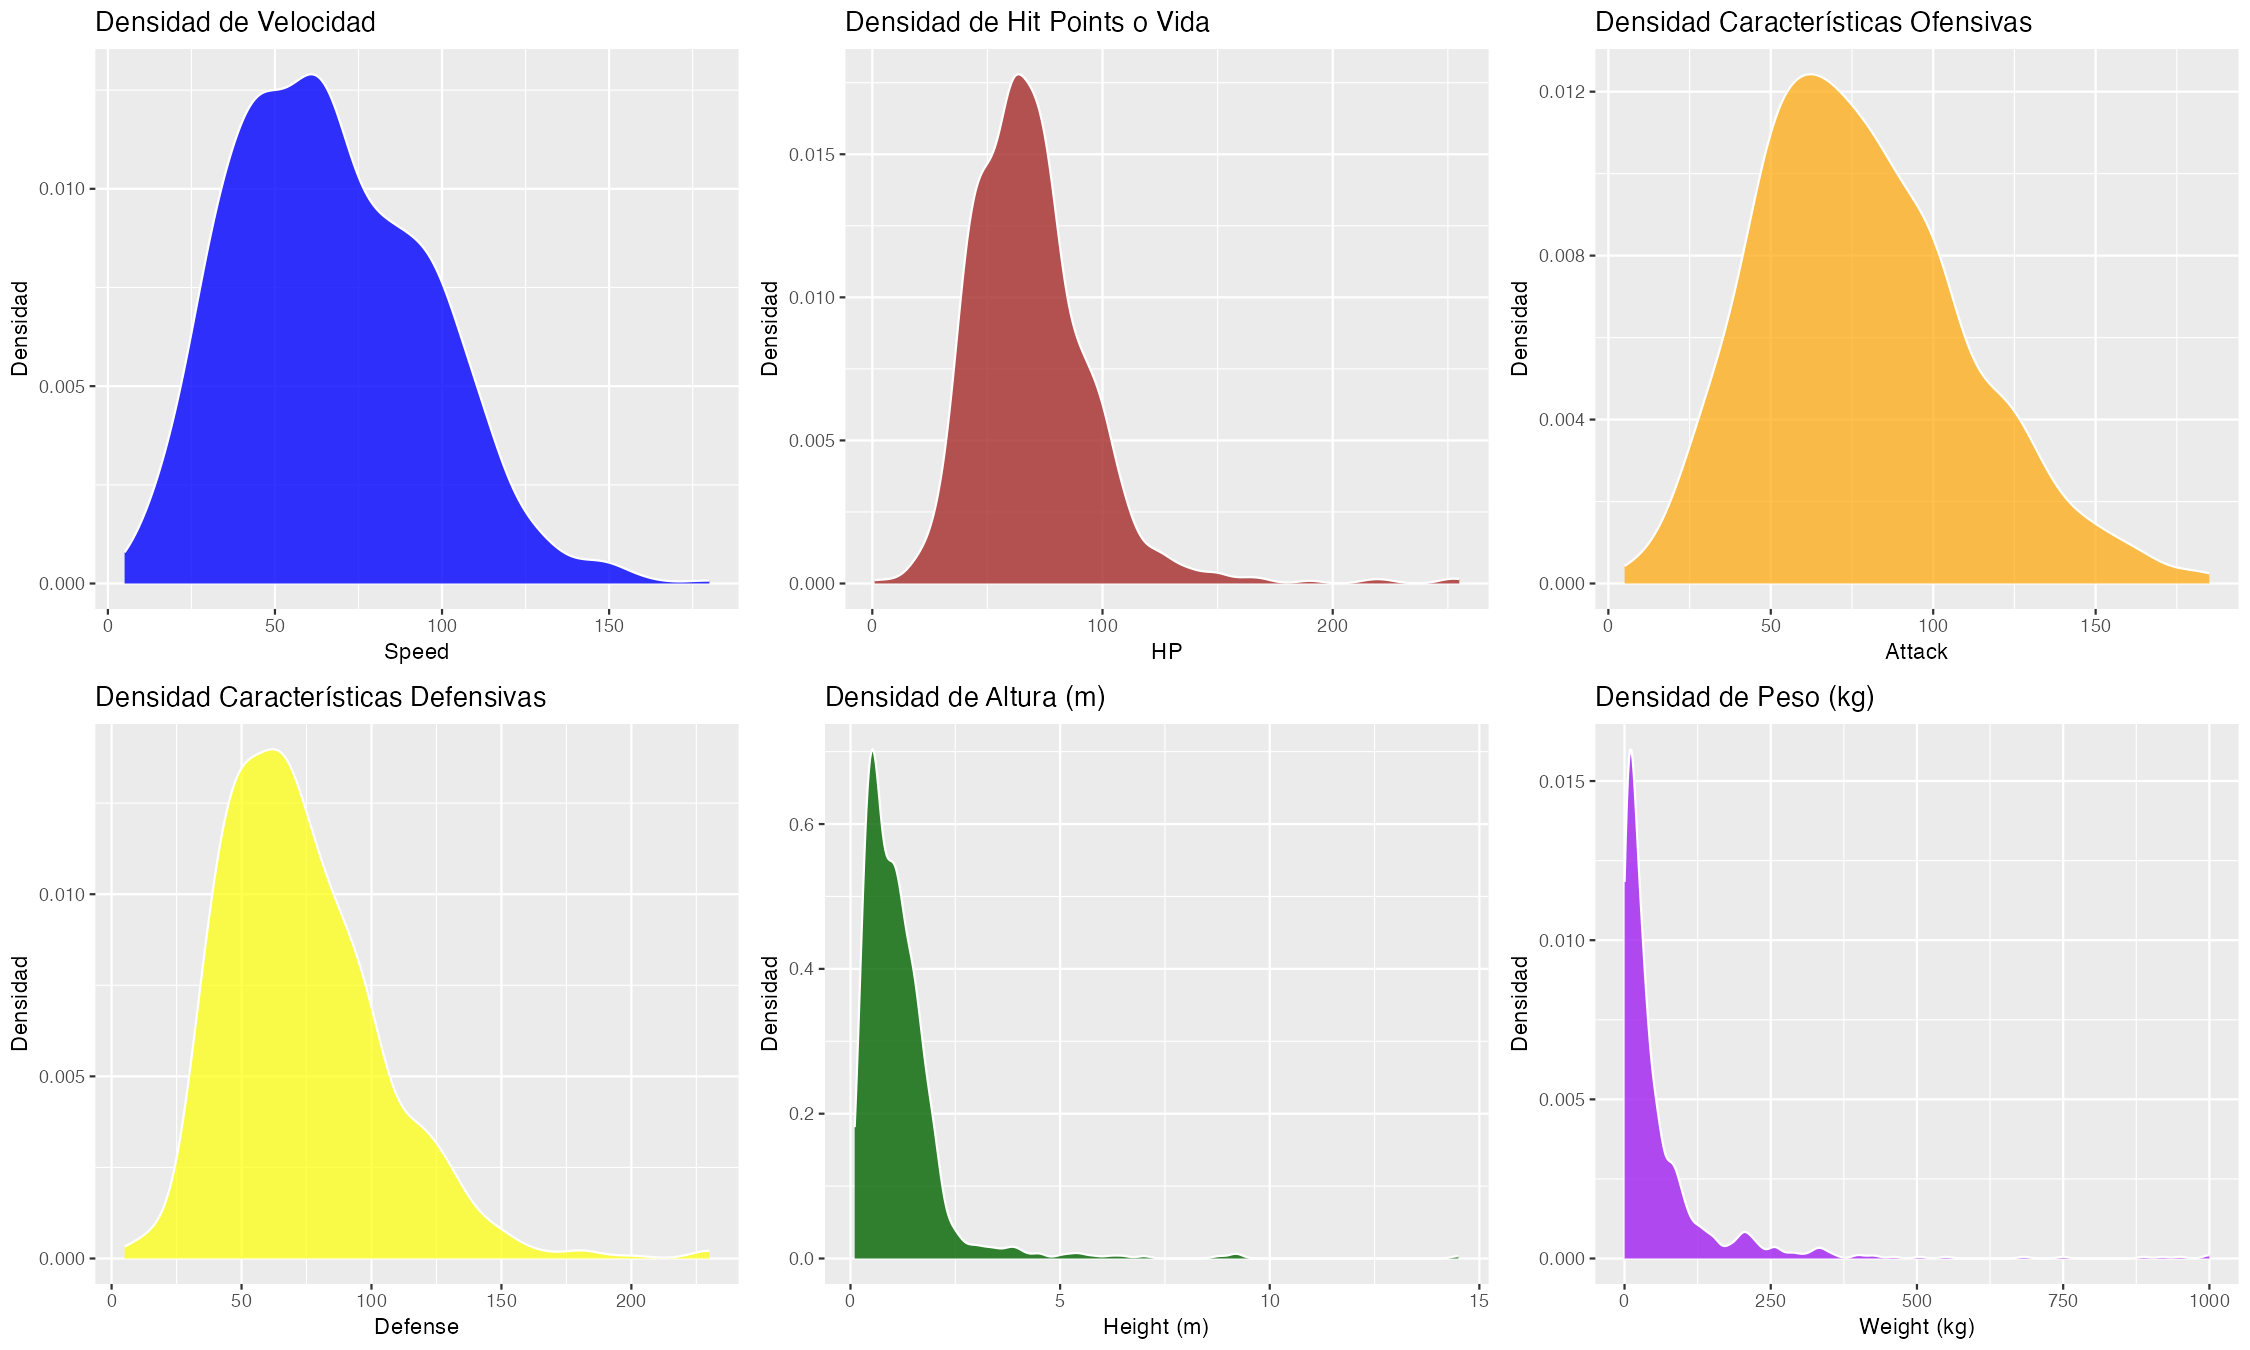
\includegraphics[width=\textwidth]{plots/density_grid_6.png}
  \caption{Grid extendido con 6 diagramas de densidad: velocidad, HP, ataque, defensa, altura y peso.
           Nótese que las distribuciones de peso y altura presentan mayor asimetría positiva.}
\end{figure}

% ============================================================
\subsection{B.2 Diagramas de Caja Avanzados}

Es posible crear boxplots que permitan comparar múltiples variables simultáneamente para diferentes
grupos. El siguiente código compara las características \texttt{hp}, \texttt{defense}, \texttt{attack},
\texttt{sp\_attack}, \texttt{sp\_defense} y \texttt{speed} entre Pokémon legendarios y no legendarios.
Para ello, los datos se convierten a formato largo (tidy) con la función \texttt{gather()} de \texttt{tidyr}.

\begin{lstlisting}[style=Rstyle]
box_plot_attr <- select(df, type1, is_legendary, hp, defense,
                        attack, sp_attack, sp_defense, speed)

box_plot_attr_leg <- filter(box_plot_attr, is_legendary == 1)
box_plot_attr_nor <- filter(box_plot_attr, is_legendary == 0)

box_plot_attr_leg_long <- gather(box_plot_attr_leg, attribute,
                                  value, -c(type1, is_legendary))
box_plot_attr_nor_long <- gather(box_plot_attr_nor, attribute,
                                  value, -c(type1, is_legendary))

bp_leg <- ggplot(data=box_plot_attr_leg_long, aes(attribute, value)) +
  geom_boxplot(fill="green4") +
  ggtitle("Pokemon Legendario")

bp_nor <- ggplot(data=box_plot_attr_nor_long, aes(attribute, value)) +
  geom_boxplot(fill="yellow2") +
  ggtitle("Pokemon No Legendario")

grid.arrange(bp_leg, bp_nor, ncol=2)
\end{lstlisting}

\begin{figure}[H]
  \centering
  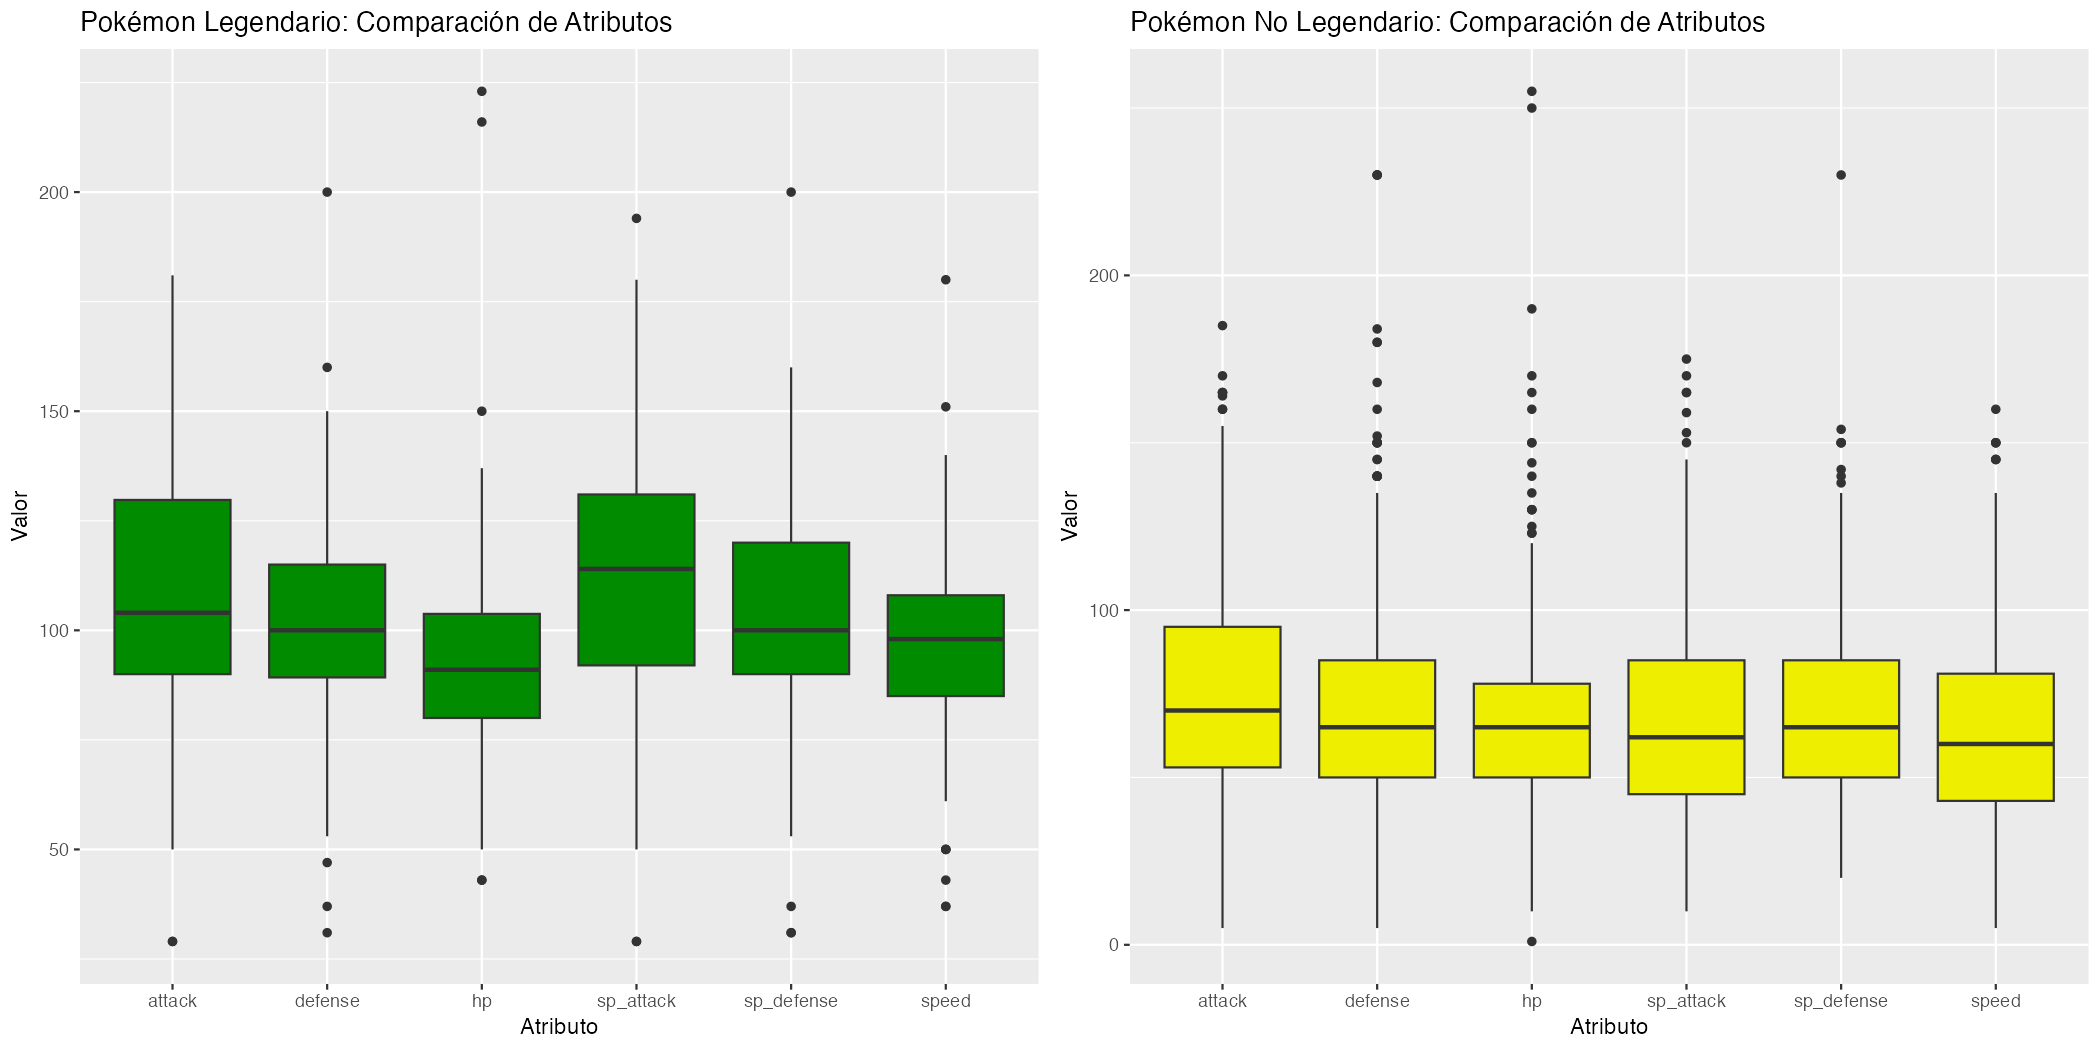
\includegraphics[width=\textwidth]{plots/boxplot_advanced.png}
  \caption{Comparación de atributos de combate entre Pokémon legendarios (izquierda, verde) y
           no legendarios (derecha, amarillo). Los legendarios presentan medianas sistemáticamente
           más altas en todos los atributos.}
\end{figure}

% ============================================================
\subsection{B.3 Mapas de Calor}

Un mapa de calor reemplaza los valores numéricos de una tabla por colores, utilizando una escala
colorimétrica continua. Esto permite identificar visualmente grupos de filas o columnas con valores
similares, facilitando la detección de tendencias en datos multidimensionales.

\textbf{Mapa de calor: Pokémon Legendarios (Type1 vs Atributo)}

Se calcula la mediana de cada atributo (\texttt{hp}, \texttt{attack}, \texttt{defense},
\texttt{sp\_attack}, \texttt{sp\_defense}, \texttt{speed}) por tipo primario, para los
Pokémon legendarios. El resultado se convierte a formato largo con \texttt{melt()} y se grafica
usando una paleta de colores \texttt{RdYlBu} (de azul = bajo, a rojo = alto).

\begin{lstlisting}[style=Rstyle]
hmap_attr <- select(df, type1, is_legendary, hp, defense,
                    attack, sp_attack, sp_defense, speed)
hmap_attr_leg <- filter(hmap_attr, is_legendary == 1)
hmap_attr_leg <- group_by(hmap_attr_leg, type1)
hmap_attr_leg <- summarise(hmap_attr_leg,
  hp=median(hp), attack=median(attack), defense=median(defense),
  sp_attack=median(sp_attack), sp_defense=median(sp_defense),
  speed=median(speed))

hmap_attr_leg_m <- melt(hmap_attr_leg)
hm.palette <- colorRampPalette(rev(brewer.pal(5, 'RdYlBu')), space='Lab')

ggplot(data=hmap_attr_leg_m, aes(type1, variable)) +
  geom_tile(aes(fill=value)) +
  ggtitle("Pokemon Legendario: Type1 - Atributo") +
  scale_fill_gradientn(colours = hm.palette(100)) +
  theme(axis.text.x = element_text(angle=90, hjust=0)) +
  coord_equal()
\end{lstlisting}

\begin{figure}[H]
  \centering
  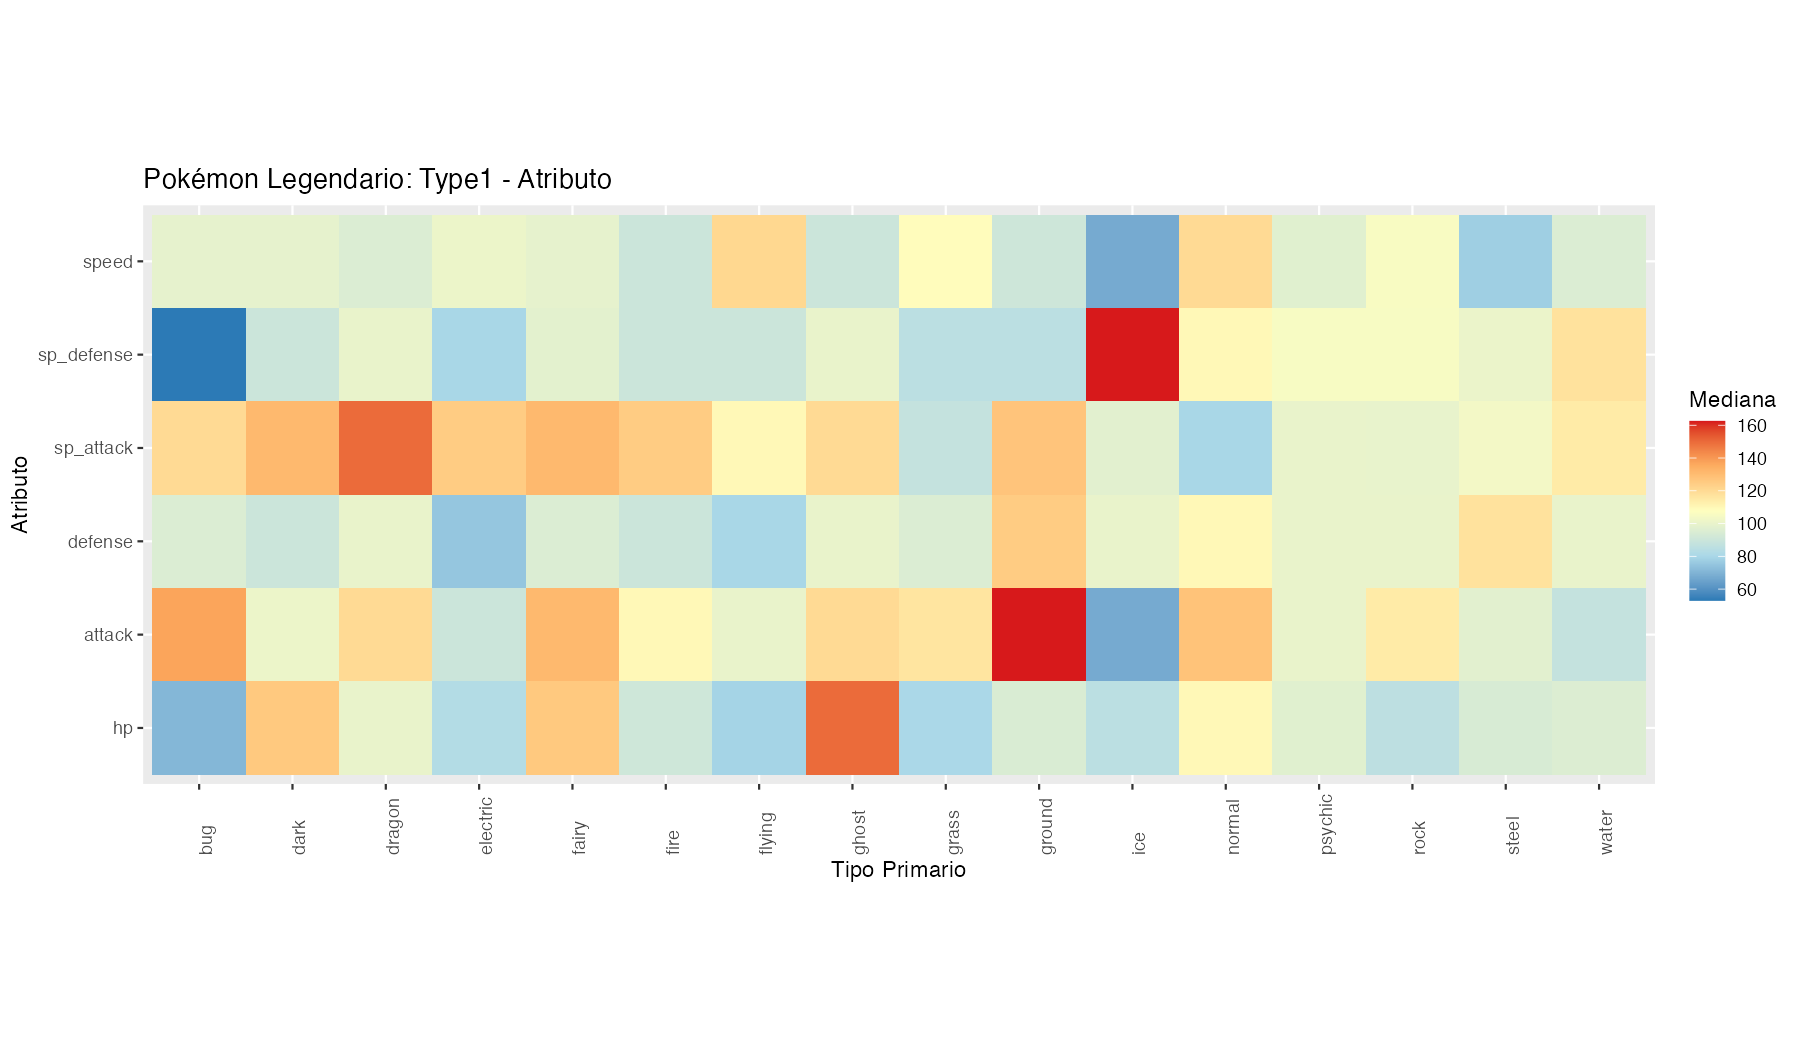
\includegraphics[width=\textwidth]{plots/heatmap_legendary.png}
  \caption{Mapa de calor de la mediana de atributos por tipo primario para Pokémon \textbf{legendarios}.
           El rojo indica valores altos y el azul valores bajos.}
\end{figure}

Se puede observar que:
\begin{itemize}
  \item Los Pokémon legendarios de tipo \textbf{hielo (ice)} tienen un valor muy alto de
    \texttt{sp\_defense}, pero un valor bajo de \texttt{speed}.
  \item Los Pokémon legendarios \textbf{terrestres (ground)} presentan un valor muy alto de \texttt{attack}.
  \item Los Pokémon legendarios de tipo \textbf{insecto (bug)} tienen un nivel muy bajo de \texttt{sp\_defense}.
\end{itemize}

\textbf{Mapa de calor: Pokémon No Legendarios (Type1 vs Atributo)}

Se construye un mapa de calor equivalente para los Pokémon no legendarios:

\begin{lstlisting}[style=Rstyle]
hmap_attr_nor <- filter(hmap_attr, is_legendary == 0)
hmap_attr_nor <- group_by(hmap_attr_nor, type1)
hmap_attr_nor <- summarise(hmap_attr_nor,
  hp=median(hp), attack=median(attack), defense=median(defense),
  sp_attack=median(sp_attack), sp_defense=median(sp_defense),
  speed=median(speed))

hmap_attr_nor_m <- melt(hmap_attr_nor)

ggplot(data=hmap_attr_nor_m, aes(type1, variable)) +
  geom_tile(aes(fill=value)) +
  ggtitle("Pokemon No Legendario: Type1 - Atributo") +
  scale_fill_gradientn(colours = hm.palette(100)) +
  theme(axis.text.x = element_text(angle=90, hjust=0)) +
  coord_equal()
\end{lstlisting}

\begin{figure}[H]
  \centering
  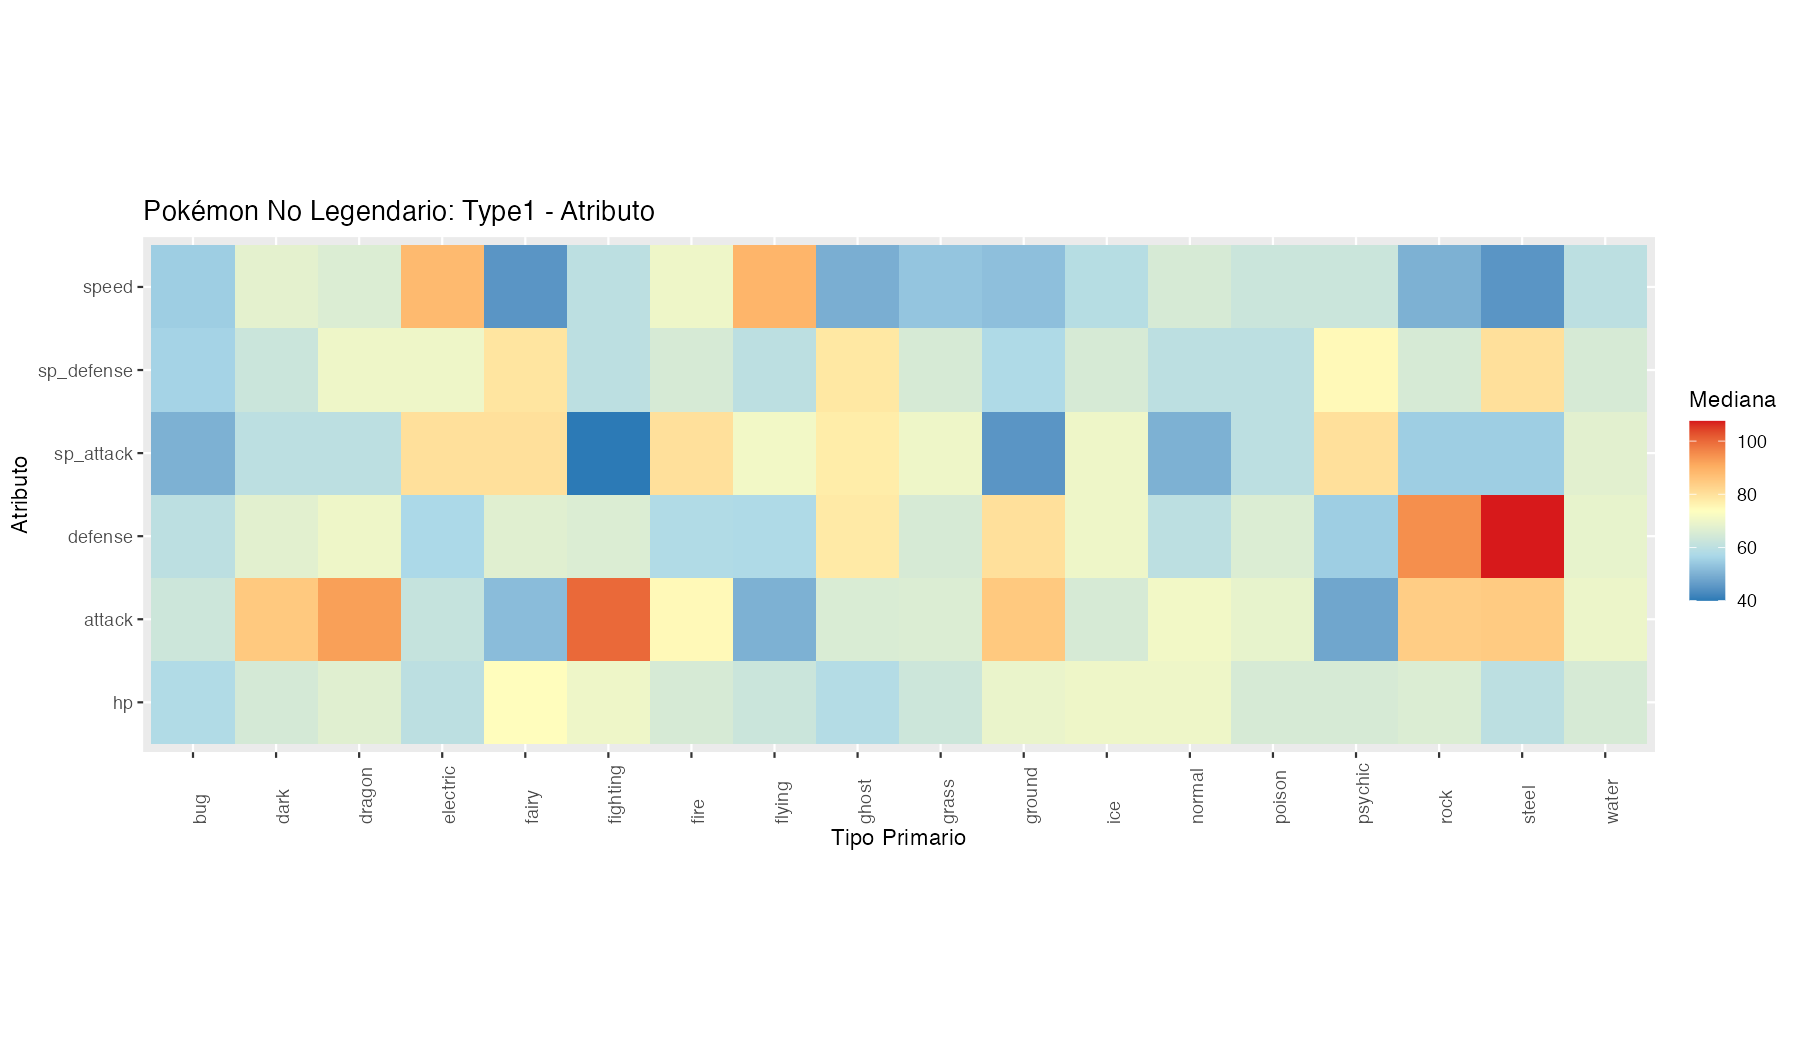
\includegraphics[width=\textwidth]{plots/heatmap_non_legendary.png}
  \caption{Mapa de calor de la mediana de atributos por tipo primario para Pokémon \textbf{no legendarios}.}
\end{figure}

En este mapa de calor se puede confirmar lo indicado en el enunciado:
\begin{itemize}
  \item[\textbf{a.}] Los Pokémon tipo \textbf{acero (steel)} tienen un alto valor de \texttt{defense},
    pero una velocidad (\texttt{speed}) muy baja.
  \item[\textbf{b.}] Los Pokémon de tipo \textbf{lucha (fighting)} tienen un alto valor de
    \texttt{attack}, pero un valor muy bajo de \texttt{sp\_attack}.
  \item[\textbf{c.}] Los Pokémon \textbf{terrestres (ground)}, de \textbf{hielo (ice)} y
    \textbf{normales (normal)} tienen niveles de HP similares entre sí.
  \item[\textbf{d.}] Los Pokémon de tipo \textbf{veneno (poison)}, \textbf{psíquico (psychic)} y
    \textbf{roca (rock)} tienen niveles de HP similar.
\end{itemize}

% ============================================================
\section{Conclusiones}
% ============================================================

A través de este laboratorio se aplicó un análisis exploratorio de datos completo sobre el
conjunto de datos de Pokémon de Kaggle con 801 entradas y 40 variables. Los principales hallazgos son:

\begin{itemize}
  \item Se detectaron \textbf{20 valores faltantes} en las variables \texttt{weight\_kg} y
    \texttt{height\_m}, distribuidos principalmente en las generaciones 1, 6 y 7, lo que indica
    posibles omisiones en la recolección de datos para ciertas generaciones.

  \item Los tipos primarios más comunes son \textbf{water}, \textbf{normal} y \textbf{grass},
    reflejando el diseño de la franquicia que favorece Pokémon acuáticos y comunes en las primeras
    etapas del juego.

  \item Solo el \textbf{8.7\%} de los Pokémon (70 de 801) son legendarios, con el tipo
    \textbf{psíquico} siendo el grupo legendario más numeroso en el tipo primario.

  \item La distribución de estadísticas como \texttt{hp}, \texttt{attack} y \texttt{speed} son
    relativamente independientes entre sí, con poca correlación lineal observada en los
    diagramas de dispersión.

  \item Los mapas de calor revelaron patrones claros de especialización por tipo: los Pokémon
    de tipo acero son lentos pero muy defensivos, los de tipo lucha son físicamente poderosos
    pero débiles en ataques especiales, y los legendarios en general superan a los no legendarios
    en todos los atributos de combate.
\end{itemize}

\end{document}
